%% =====================================================================
%% From Passive Members to Self-Aware Steel Structures
%% Target journal: Automation in Construction (Elsevier, ISSN 0926-5805)
%% Class: elsarticle (numbered references)
%% Compile: latexmk -pdf -interaction=nonstopmode main.tex
%% =====================================================================
\documentclass[preprint,12pt]{elsarticle}

\usepackage{amssymb,amsmath}
\usepackage{booktabs}
\usepackage{array}
\usepackage{tabularx}
\usepackage{multirow}
\usepackage{xcolor}
\usepackage{tikz}
\usetikzlibrary{positioning,arrows.meta,shapes.geometric,shapes.misc,calc,fit,backgrounds,decorations.pathmorphing}
\usepackage{pgfplots}
\pgfplotsset{compat=1.18}
\usepgfplotslibrary{groupplots}

%% Elsevier-friendly colour palette (used by the TikZ/pgfplots figures)
\definecolor{elsB1}{HTML}{08306B}
\definecolor{elsB2}{HTML}{2171B5}
\definecolor{elsB3}{HTML}{6BAED6}
\definecolor{elsB4}{HTML}{C6DBEF}
\definecolor{elsC1}{HTML}{66C2A5}
\definecolor{elsC2}{HTML}{FC8D62}

%% For double line spacing during review, use the [review] class option.
%% \usepackage{lineno}\linenumbers

\journal{Automation in Construction}

\begin{document}

\begin{frontmatter}

\title{From Passive Members to Self-Aware Steel Structures: A Digital-Twin and
Machine-Learning Framework for Structural Cognition and Autonomous Health Monitoring}

\author[inst1]{[First Author]\corref{cor1}}
\ead{first.author@institution.edu}

\author[inst1]{[Second Author]}

\cortext[cor1]{Corresponding author.}

\affiliation[inst1]{organization={[Department]},
            addressline={[Street address]},
            city={[City]},
            postcode={[Postcode]},
            state={[State]},
            country={[Country]}}

\begin{abstract}
Steel structures are conventionally treated as passive load-resisting members
whose integrity is verified by periodic inspection. Structural health monitoring
(SHM) added continuous measurement, yet many deployments still stop at data
acquisition, leaving interpretation to offline analysis. This paper proposes a
conceptual framework and reference architecture for the Self-Aware Steel
Structure, which perceives, processes, interprets and autonomously reports its
own mechanical state through a permanent link to a continuously updated digital
twin. We introduce the paradigm of Structural Cognition and an operational
six-level scale (L0--L5) of structural self-awareness mapped onto the Rytter
damage hierarchy. A five-layer architecture couples distributed multi-sensor
acquisition, a finite-element digital twin, a machine-learning cognition layer
(unsupervised novelty detection with autoencoders, supervised classification, and
LSTM temporal modelling) and a governed decision layer. A braced
square-hollow-section frame under rotating-unbalance excitation is specified as
the validation testbed, advancing cognitive digital twins and autonomous
predictive maintenance of steel infrastructure.
\end{abstract}

\begin{graphicalabstract}
\centering
\resizebox{0.96\linewidth}{!}{% Body-only graphical abstract, \input by main.tex frontmatter.
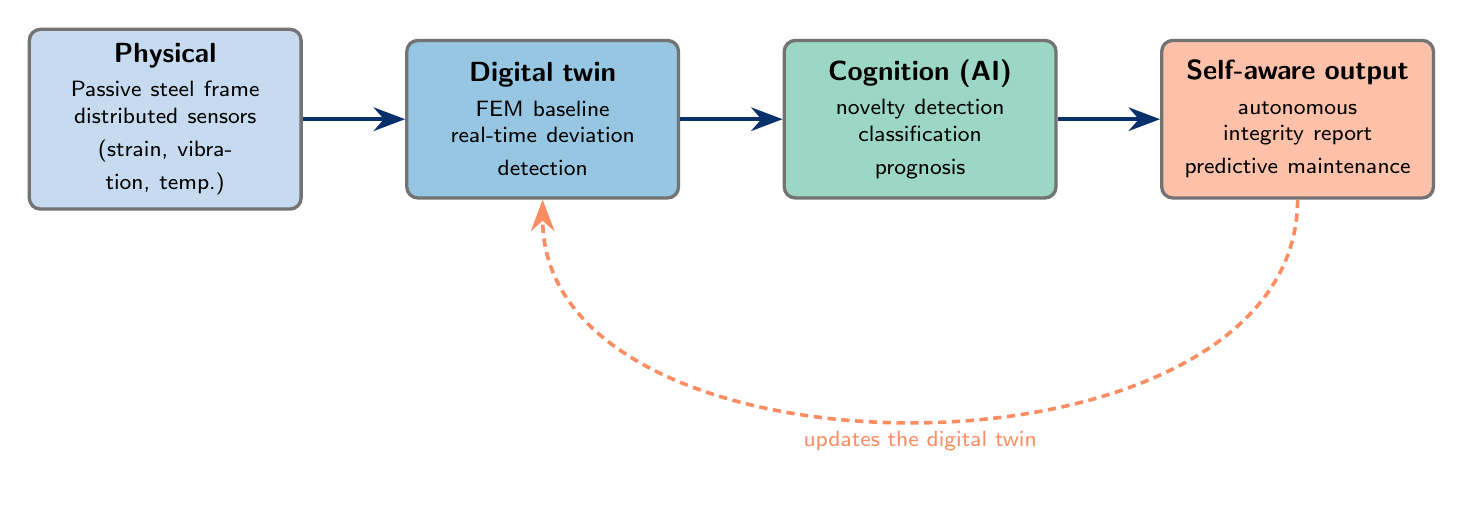
\begin{tikzpicture}[
  every node/.style={font=\sffamily},
  stage/.style={rectangle, rounded corners=4pt, draw=black!55, very thick,
                text width=3.1cm, minimum height=2.0cm, align=center, inner sep=5pt},
  arr/.style={-{Stealth[length=4mm]}, line width=1.3pt, elsB1}
]
  \node[stage, fill=elsB4] (phys)
        {\textbf{Physical}\\[3pt]\footnotesize Passive steel frame\\ distributed sensors\\ (strain, vibration, temp.)};
  \node[stage, fill=elsB3!70, right=1.3cm of phys] (twin)
        {\textbf{Digital twin}\\[3pt]\footnotesize FEM baseline\\ real-time deviation\\ detection};
  \node[stage, fill=elsC1!65, right=1.3cm of twin] (cog)
        {\textbf{Cognition (AI)}\\[3pt]\footnotesize novelty detection\\ classification\\ prognosis};
  \node[stage, fill=elsC2!55, right=1.3cm of cog] (out)
        {\textbf{Self-aware output}\\[3pt]\footnotesize autonomous\\ integrity report\\ predictive maintenance};
  \draw[arr] (phys) -- (twin);
  \draw[arr] (twin) -- (cog);
  \draw[arr] (cog) -- (out);
  \draw[-{Stealth[length=4mm]}, line width=1.3pt, densely dashed, elsC2]
        (out.south) to[out=270,in=270]
        node[below, font=\footnotesize\sffamily, elsC2]{updates the digital twin} (twin.south);
\end{tikzpicture}
}
\end{graphicalabstract}

\begin{highlights}
\item Self-Aware Steel Structure paradigm shifts members from passive to cognitive.
\item Structural Cognition lets a structure interpret and report its own state.
\item Five-layer architecture couples sensing, FEM digital twin and learning.
\item Supervised and unsupervised AI target stiffness loss and bolt-loosening detection.
\item SHS braced-frame testbed enables autonomous predictive maintenance of steel.
\end{highlights}

\begin{keyword}
Self-aware structures \sep Structural cognition \sep Digital twin \sep
Structural health monitoring \sep Machine learning \sep
Autonomous damage detection \sep Steel structures
\end{keyword}

\end{frontmatter}

%% ===================== Main text =====================
\section{Introduction}\label{sec:intro}

Steel structures have historically been conceived as passive load-resisting systems. A frame, a truss or a braced industrial skeleton is designed to a code-specified set of limit states, erected, and thereafter assumed to behave as drawn for the remainder of its service life. Within this paradigm, knowledge of the structure's actual condition is acquired discontinuously, through periodic visual inspection and occasional non-destructive evaluation, and is mediated entirely by human judgement. The structure itself contributes nothing to the assessment of its own integrity: it carries load, accumulates damage silently, and waits to be examined. This passive model has well-known limitations. Inspections are infrequent, labour-intensive and costly; they favour accessible and visible regions; and they capture the state of the structure only at isolated instants, leaving long intervals during which deterioration, fatigue crack growth, support settlement or the progressive loosening of bolted connections may develop undetected \citep{avci2021review}.

Structural Health Monitoring (SHM) emerged precisely to overcome the discontinuity of inspection. SHM is the process of implementing a damage detection strategy for aerospace, civil and mechanical infrastructure by observing a structure over time through periodically sampled response measurements, extracting damage-sensitive features and statistically analysing those features to determine the current state of system health \citep{farrar2013shm,farrar2007introduction}. The premise is physically grounded: damage is a change in the material or geometric properties of a system, including changes to boundary conditions and connectivity, that alters its stiffness, mass or energy-dissipation characteristics and therefore its measured dynamic response \citep{farrar2013shm}. The natural vibration properties of a structure depend only on its mass and stiffness, so that its natural frequencies and mode shapes are fixed by these two quantities alone \citep{chopra2017dynamics}; any stiffness loss is, in principle, observable as a measurable shift in frequencies, mode shapes and damping. The textbook precedent of period lengthening accompanying stiffness reduction confirms that monitored modal parameters genuinely track structural condition \citep{chopra2017dynamics}.

Yet most deployed SHM systems stop short of their own promise. They excel at instrumentation, acquisition, storage and transmission of data, but the interpretation of those data, the conversion of raw signals into a statement about the structure's health, is too often performed off the structure, by human experts and after the fact. Automated and near-real-time SHM methods do exist \citep{avci2021review,he2022integrated}; what remains uncommon is interpretation embedded in the structure itself, together with an explicit measure of how autonomously it acts. This reflects a structural imbalance in the field itself: feature extraction and, especially, the statistical modelling that discriminates damage states have historically received far less attention than data acquisition, even though it is here that sensor data become damage information \citep{farrar2013shm}. A sensor cannot measure damage directly; without intelligent feature extraction and statistical classification, the structure remains mute \citep{farrar2013shm}. The result is a generation of monitored structures that are richly instrumented but cognitively inert: they sense, but they do not understand.

A convergence of enabling technologies now makes it feasible to close this gap. Embedded and distributed sensing, using dense arrays of strain gauges, triaxial accelerometers, temperature sensors, displacement transducers and inclinometers fused across heterogeneous channels \citep{farrar2013shm}, provides continuous, multi-physics observation. The finite element method supplies a rigorous physical baseline: assembling element stiffness matrices into a global model and solving the free-vibration eigenproblem yields the natural frequencies and mode shapes against which measured behaviour can be compared \citep{cook2002fea}. The FE model is simulation, not reality, and its disagreement with experiment is itself diagnostic \citep{cook2002fea}, a property that turns model--data correlation into a continuous deviation detector. Machine learning supplies the interpretive layer: supervised methods such as Random Forest, Support Vector Machines and Artificial Neural Networks classify damage type and severity, while unsupervised methods such as autoencoders and recurrent LSTM networks learn healthy behaviour and flag novelty \citep{naser2023ml,brunton2019data,wangcha2022unsupervised}. Data-driven dimensionality reduction (SVD/PCA), equation-free modal extraction (DMD) and physics-informed learning provide the algorithmic machinery to fuse model and measurement into a single predictive object, the digital twin \citep{brunton2019data,chiachio2022structural}. Embedded within an Industry 4.0 ecosystem of continuous acquisition, edge processing and connectivity, these elements together permit a permanent, real-time link between a physical structure and its digital representation \citep{li2025edge,zou2026deep}.

Building on this convergence, we introduce the concept of the \textbf{Self-Aware Steel Structure}: a structure able to perceive, process, interpret and continuously report its own mechanical state. We name the resulting paradigm \textbf{Structural Cognition}. Under it, a steel structure ceases to be merely a load-resisting element and becomes an intelligent system that interprets its own behaviour, recognises changes in operational condition, identifies stiffness loss and bolted-connection loosening, detects progressive damage, and autonomously assesses its integrity, advancing along the damage-state hierarchy from existence and location toward type, severity and prognosis \citep{farrar2013shm}.

The research gap addressed by this paper is conceptual and architectural rather than purely instrumental. Digital twins, finite-element models and machine learning have already been combined for structural monitoring, including structural digital-twin formulations \citep{chiachio2022structural}, deep-learning- and digital-twin-driven SHM \citep{zou2026deep}, and autonomous, distributed monitoring architectures \citep{li2025edge,mariniello2025enhancing}. What these works do not provide is an explicit, operational scale of \textit{how autonomously} a structure interprets and acts on its own state, together with a steel-specific architecture and protocol that operationalise it. The objective of this paper is to supply that missing layer, whose architecture is summarised in Fig.~\ref{fig:arch}. This is a conceptual framework and review paper: it proposes the Structural Cognition paradigm, an operational six-level taxonomy (L0--L5) of structural self-awareness, a reference architecture for Self-Aware Steel Structures, and a detailed experimental specification centred on an instrumented three-dimensional braced frame of square hollow sections excited by a controlled rotating-unbalance system. The paper does not report empirical measurements; the experimental campaign is described as a planned validation pathway. Its contributions are threefold: (i) the formal articulation of Structural Cognition together with an operational L0--L5 maturity scale that moves SHM from data acquisition toward autonomous interpretation; (ii) a reference architecture integrating multi-sensor fusion, a continuously updated digital twin and a supervised/unsupervised learning layer grounded in established theory, whose five foundational pillars are listed in Table~\ref{tab:pillars} \citep{farrar2013shm,brunton2019data,chopra2017dynamics,naser2023ml,cook2002fea}; and (iii) a structured, auditable six-step methodology and experimental specification for realising and validating a Self-Aware Steel Structure.

The remainder of the paper is organised as follows. Section~\ref{sec:background} reviews the theoretical foundations of SHM, structural dynamics, finite element modelling, digital twins and machine learning that underpin Structural Cognition. Section~\ref{sec:paradigm} defines the Self-Aware Steel Structure and the Structural Cognition paradigm conceptually. Section~\ref{sec:architecture} presents the proposed reference architecture. Section~\ref{sec:methodology} details the experimental methodology and instrumented testbed. Section~\ref{sec:ml} describes the digital-twin implementation and the learning layer for autonomous integrity assessment. Section~\ref{sec:discussion} discusses implications, limitations and open challenges, and Section~\ref{sec:conclusions} concludes.

\begin{table}[htbp]
\centering
\caption{Theoretical foundations of the Structural Cognition framework and their role in the proposed architecture.}
\label{tab:pillars}
\begin{tabularx}{\linewidth}{@{}l l X@{}}
\toprule
\textbf{Domain} & \textbf{Source} & \textbf{Contribution to the framework} \\
\midrule
Structural health monitoring & \citep{farrar2013shm} & Statistical pattern recognition paradigm, Rytter damage hierarchy, SHM axioms, novelty detection, environmental normalisation \\
Structural dynamics & \citep{chopra2017dynamics} & Modal parameters as condition-sensitive features; resonance; damping estimation; vibration-based monitoring \\
Finite element analysis & \citep{cook2002fea} & Physics baseline; free-vibration eigenproblem; model updating; verification and validation \\
Data-driven modelling & \citep{brunton2019data} & Dimensionality reduction (SVD/PCA), reduced-order models, DMD, autoencoders and LSTM \\
Machine learning in civil engineering & \citep{naser2023ml} & ML workflow; Random Forest, SVM, ANN; evaluation metrics; explainability; data-scarcity remedies \\
\bottomrule
\end{tabularx}
\end{table}

\begin{figure}[htbp]
\centering
\resizebox{\linewidth}{!}{%
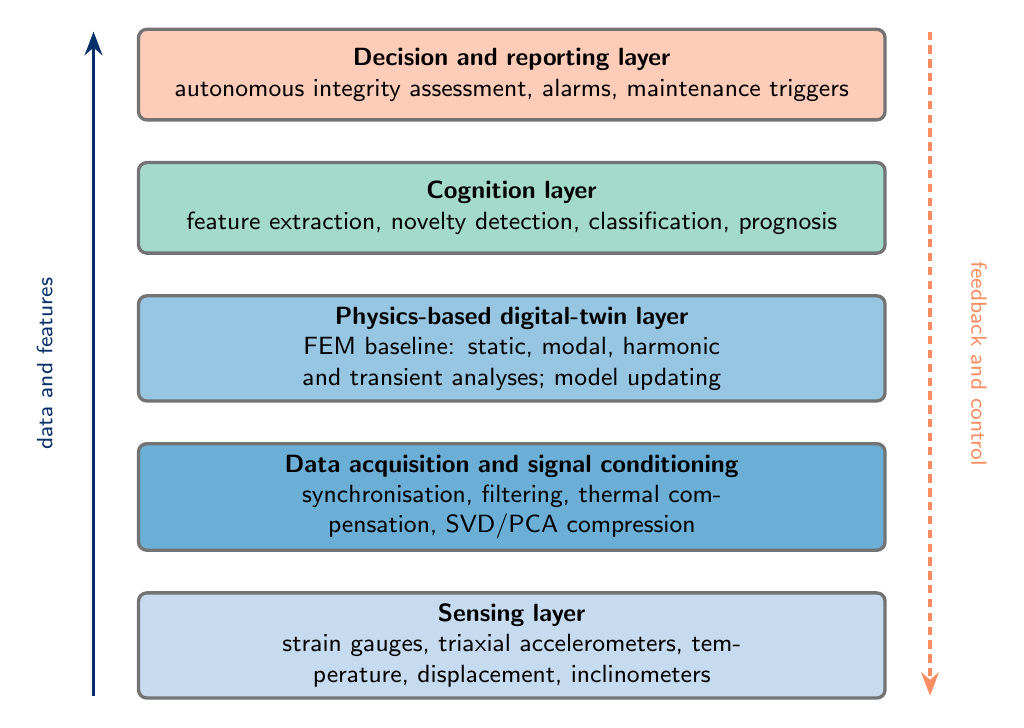
\begin{tikzpicture}[
  every node/.style={font=\small\sffamily},
  layer/.style={rectangle, rounded corners=3pt, draw=black!55, very thick,
                text width=9.2cm, minimum height=1.15cm, align=center, inner sep=4pt},
  flowup/.style={-{Stealth[length=3mm]}, very thick, elsB1},
  flowdn/.style={-{Stealth[length=3mm]}, very thick, densely dashed, elsC2}
]
  \node[layer, fill=elsB4]                       (l1) {\textbf{Sensing layer}\\ strain gauges, triaxial accelerometers, temperature, displacement, inclinometers};
  \node[layer, fill=elsB3, above=0.5cm of l1]    (l2) {\textbf{Data acquisition and signal conditioning}\\ synchronisation, filtering, thermal compensation, SVD/PCA compression};
  \node[layer, fill=elsB3!70, above=0.5cm of l2] (l3) {\textbf{Physics-based digital-twin layer}\\ FEM baseline: static, modal, harmonic and transient analyses; model updating};
  \node[layer, fill=elsC1!60, above=0.5cm of l3] (l4) {\textbf{Cognition layer}\\ feature extraction, novelty detection, classification, prognosis};
  \node[layer, fill=elsC2!45, above=0.5cm of l4] (l5) {\textbf{Decision and reporting layer}\\ autonomous integrity assessment, alarms, maintenance triggers};
  \draw[flowup] ($(l1.south west)+(-0.55,0.05)$) -- ($(l5.north west)+(-0.55,-0.05)$);
  \node[rotate=90, anchor=south, font=\footnotesize\sffamily, elsB1]
        at ($(l1.south west)!0.5!(l5.north west)+(-0.95,0)$) {data and features};
  \draw[flowdn] ($(l5.north east)+(0.55,-0.05)$) -- ($(l1.south east)+(0.55,0.05)$);
  \node[rotate=-90, anchor=south, font=\footnotesize\sffamily, elsC2]
        at ($(l5.north east)!0.5!(l1.south east)+(0.95,0)$) {feedback and control};
\end{tikzpicture}}
\caption{Five-layer reference architecture of a Self-Aware Steel Structure. Sensor data are progressively transformed into an autonomous integrity assessment (left, bottom-up), while diagnosed conditions feed back to update the healthy baseline, the digital twin and the learning models (right, top-down).}
\label{fig:arch}
\end{figure}


\section{Background and related work}\label{sec:background}

The proposed Self-Aware Steel Structure builds on three mature bodies of knowledge that have so far evolved largely in parallel. Structural health monitoring (SHM) is the discipline for inferring structural condition from measured response. Data-driven modeling compresses high-dimensional measurements into interpretable low-dimensional representations of system behavior. Machine learning (ML) supplies a practical toolset for civil and structural engineering. This section reviews these foundations and clarifies the terminology and assumptions on which the remainder of the paper relies. The recurring theme is that each field provides a necessary but individually insufficient ingredient: SHM defines \textit{what} must be inferred and \textit{why} a baseline comparison is required, data-driven modeling defines \textit{how} raw multi-channel signals are reduced to features that a digital representation can reason about, and ML defines \textit{how} those features are mapped to actionable statements about structural integrity \citep{farrar2013shm,brunton2019data,naser2023ml}. The novelty of the present work, developed in later sections, lies in fusing these ingredients into a structure that interprets its own state rather than merely transmitting data.

\subsection{Structural health monitoring as statistical pattern recognition}\label{subsec:shm-spr}

The canonical formulation of SHM frames damage detection as a statistical pattern recognition (SPR) problem \citep{farrar2013shm}. In this view, SHM is the process of implementing a damage detection strategy by observing a structure over time through periodically spaced response measurements, extracting damage-sensitive features from those measurements, and statistically analyzing the features to determine the current state of system health \citep{farrar2007introduction}. The process is organized into four integrated parts: (i) operational evaluation, which establishes the life-safety and economic justification for monitoring, defines what constitutes damage for the system at hand, and identifies the operational and environmental conditions under which data will be acquired; (ii) data acquisition, which selects excitation methods, sensor types, numbers and locations, and the hardware for acquisition, storage and transmittal; (iii) feature selection and extraction, which identifies low-dimensional quantities that are sensitive to damage yet robust to confounding influences; and (iv) statistical modeling for feature discrimination, in which learning algorithms operate on the extracted features to quantify the damage state \citep{farrar2013shm}. Data normalization, cleansing, compression and fusion are embedded within these parts, and ML enters primarily in the third and fourth.

Two foundational principles underpin this paradigm and are inherited directly by the present framework. First, damage assessment is intrinsically a \textit{comparison between two states} of the system, one of which is assumed to represent an undamaged baseline; damage itself is defined as a change to the material or geometric properties of a system, including changes to boundary conditions and connectivity, that adversely affects current or future performance \citep{farrar2013shm}. The loosening of a bolted connection is an explicit example: it alters connectivity and typically adds energy dissipation, which manifests as an increase in measured damping. Second, sensors cannot measure damage directly. Feature extraction and statistical classification are required to convert sensor data into damage information, and without intelligent feature extraction the most damage-sensitive measurements are also the most sensitive to benign operational and environmental variability \citep{farrar2013shm}.

The depth of diagnosis achievable is organized by the Rytter hierarchy, which orders the damage-identification questions by increasing knowledge of the damage state: existence, location, type, severity (extent), and prognosis \citep{farrar2013shm}. This hierarchy maps onto the supervised/unsupervised distinction that governs the choice of learning algorithm. Unsupervised learning, which builds a model of a single healthy class and tests new data for consistency with that class, can typically establish the \textit{existence} of damage and sometimes its \textit{location}; this leads naturally to novelty and outlier detection, the appropriate paradigm when only undamaged data are available, as is usually the case because deliberately damaging high-value structures is impractical \citep{sohn2003statistical,wangcha2022unsupervised}. Determining the \textit{type} and \textit{severity} of damage generally requires supervised learning trained on labeled examples from both healthy and damaged states \citep{farrar2013shm,figueiredo2010machine}. A central practical challenge is data normalization: separating response changes caused by benign operational and environmental variability, such as temperature-induced stiffness change, from those caused by damage, so that environmental fluctuation is not mistaken for structural deterioration and reported as a false positive \citep{figueiredo2010machine}. The classification of healthy versus anomalous behavior must therefore minimize both false-positive and false-negative diagnoses, whose costs may be weighted very differently \citep{farrar2013shm}.

\subsection{Data-driven modeling and reduced-order representations}\label{subsec:datadriven}

Measurements from distributed sensor networks are high-dimensional, yet the dynamics they capture typically evolve on a low-dimensional manifold, exhibiting dominant low-dimensional patterns \citep{brunton2019data}. The singular value decomposition (SVD) provides a systematic, numerically stable, and entirely data-driven way to extract these dominant correlations, yielding a hierarchical representation in which the left singular vectors are the dominant spatial patterns and the ordered singular values quantify their energy content. Principal component analysis (PCA) and proper orthogonal decomposition (POD) are computed directly from the SVD of the mean-subtracted data matrix, and the SVD furnishes the optimal low-rank approximation of a data set \citep{brunton2019data}. For the present framework, this supplies the mechanism for compressing distributed strain and acceleration streams into a few dominant modes and for defining a compact, low-dimensional baseline of healthy behavior against which deviations can be flagged.

Several complementary data-driven methods extend this idea toward dynamics. Dynamic mode decomposition (DMD) identifies spatio-temporal coherent structures from measurement snapshots and, unlike SVD/POD, associates each mode with a temporal eigenvalue encoding an oscillation frequency and a growth or decay rate; DMD is purely data-driven, requires no knowledge of the governing equations, and applies equally to experimental and numerical data \citep{brunton2019data}. The sparse identification of nonlinear dynamics (SINDy) complements this by discovering interpretable governing equations through sparse regression over a candidate function library, recovering the few active terms that describe the dynamics \citep{brunton2019data}. Reduced-order models (ROMs) project high-dimensional dynamics onto a few dominant modes for rapid evaluation, and can be coupled with sparse, optimally placed sensors to reconstruct the full field from a limited number of measurements, which provides a principled basis for numerical-analysis-driven sensor placement \citep{brunton2019data,tan2020sensorplacement,hassani2023sensorplacement}. Autoencoders learn a nonlinear latent representation by mapping an input through an encoder to a latent space and reconstructing it through a decoder; a linear autoencoder reduces to the SVD/POD basis, connecting deep learning to PCA, and the reconstruction error of a model trained on healthy data provides a natural residual that grows under abnormal conditions, an indicator well suited to anomaly detection \citep{brunton2019data}. Recurrent architectures, in particular long short-term memory (LSTM) networks, are designed to exploit the temporal structure of sequential data and can learn and reproduce the evolution of dynamical systems from short windows of observations \citep{brunton2019data}.

\subsection{Machine learning in civil and structural engineering}\label{subsec:ml-civil}

Within civil engineering, ML is best understood as a staged workflow comprising data collection, model development (training), model evaluation, and model optimization, in which an algorithm learns the mapping between input features and a target response \citep{naser2023ml}. This framing explicitly motivates SHM applications, in which sensor networks continuously measure and record information over the service life of a structure. Problems are partitioned into supervised learning, encompassing regression for numeric targets such as stress or displacement and classification for categorical targets such as discrete damage levels (for example, minor damage, major damage, and collapse), and unsupervised learning, which discovers the underlying structure of unlabeled data through clustering, dimensionality reduction, and anomaly detection \citep{naser2023ml}. Because labeled damaged-state data are scarce in SHM, semi-supervised variants and synthetic data generation are relevant, as is the use of a validated finite-element model run as a parametric study to generate augmented, hybrid (real plus simulated) datasets for training, although experimental data are generally favored over purely synthetic data \citep{naser2023ml,karaaslan2021attention}.

The algorithms named in the proposed AI layer are well established in this context. Random Forest is a non-parametric ensemble of decision trees that aggregates outcomes by averaging for regression or majority voting for classification and makes no assumption about the functional form of the feature--target relationship \citep{naser2023ml}. Support vector machines separate classes using a margin-maximizing hyperplane and accommodate nonlinearity through kernel functions such as the radial basis function, with a regression variant (SVR) \citep{naser2023ml}. Artificial neural networks arrange neurons in layers connected through differentiable activation functions and are trained by back-propagation and gradient descent; networks with multiple hidden layers constitute deep learning, and recurrent networks address sequential data, with LSTM motivated by the vanishing-gradient problem of plain recurrent networks \citep{naser2023ml}. Rigorous evaluation is essential: reporting several independent performance and error metrics, using confusion matrices, ROC curves, precision, recall, F1 and balanced accuracy for classification, and adopting stratified $k$-fold cross-validation guards against the bias of simple ratio sampling and against overfitting and underfitting \citep{naser2023ml}. The trustworthiness of an autonomous integrity assessment depends on explainability: permutation-based feature importance, partial dependence plots, SHAP and LIME provide traceable, physics-checkable explanations of why a model reaches a given diagnosis, moving beyond black-box prediction toward interpretable damage indicators \citep{naser2023ml}. Together, these methods supply the analytical machinery on which the cognitive layer of the proposed framework is built, while the data-scarcity remedies and explainability tools directly address the practical obstacles to deploying it on real steel infrastructure \citep{avci2021review}.

\subsection{Structural dynamics and vibration-based monitoring}\label{subsec:dynamics}

The premise that links a steel structure's measurable vibration response to its mechanical condition rests on the classical theory of structural dynamics. For a single-degree-of-freedom (SDOF) idealization, the equation of motion assembles inertia, damping and elastic restoring forces under dynamic equilibrium, $m\ddot{u} + c\dot{u} + ku = p(t)$ \citep{chopra2017dynamics}. Free undamped vibration of this system is simple harmonic motion whose natural circular frequency is $\omega_n = \sqrt{k/m}$, with the corresponding natural period $T_n = 2\pi/\omega_n$ and cyclic frequency $f_n = \omega_n/2\pi$. A property of central importance to monitoring follows directly: the natural vibration characteristics depend only on the mass and stiffness of the structure and not on the excitation. Consequently, of two systems of equal mass the stiffer one exhibits the higher natural frequency, and any reduction in stiffness, whether from yielding, cracking, support degradation or bolted-connection loosening, is in principle observable as a downward shift in the measured natural frequencies \citep{chopra2017dynamics,avci2021review}.

Real steel structures possess many degrees of freedom, and their dynamics are described by the matrix eigenvalue problem $\mathbf{k}\boldsymbol{\phi}_n = \omega_n^2 \mathbf{m}\boldsymbol{\phi}_n$, whose nontrivial solutions require $\det(\mathbf{k} - \omega_n^2\mathbf{m}) = 0$ \citep{chopra2017dynamics}. Because the mass and stiffness matrices are symmetric and positive definite, this characteristic equation yields $N$ real positive eigenvalues, ordered $\omega_1 < \omega_2 < \cdots < \omega_N$, each associated with a natural mode shape $\boldsymbol{\phi}_n$ describing a fixed deflected configuration in which all degrees of freedom vibrate in phase. The modes are orthogonal with respect to both mass and stiffness, which permits the coupled equations of a classically (proportionally) damped system to be transformed into $N$ independent modal SDOF equations and the total response to be recovered by modal superposition \citep{chopra2017dynamics}. The compact triplet of modal parameters, natural frequencies $\omega_n$, mode shapes $\boldsymbol{\phi}_n$ and modal damping ratios $\zeta_n$, therefore constitutes a physically interpretable fingerprint of the structure's current stiffness and mass distribution, and it is precisely this fingerprint that a self-aware structure must continuously identify and compare against a healthy baseline.

Damping characterizes energy dissipation through the ratio $\zeta = c/c_{cr}$; for most real structures it lies below 20\% and typically amounts to only a few percent, slightly reducing the damped frequency to $\omega_D = \omega_n\sqrt{1-\zeta^2}$ \citep{chopra2017dynamics}. Damping is generally not deducible from geometry and material alone but determined experimentally, for instance from the half-power (3~dB) bandwidth of the frequency-response curve, $\zeta = (f_b - f_a)/2f_n$, which is evaluable without knowledge of the applied force magnitude. Measured damping is also amplitude-dependent and tends to increase when a structure is driven into damaging regimes, a behavior with direct consequences for distinguishing healthy from abnormal states. The empirical precedent of the Millikan Library is instructive: at the larger amplitudes of the San Fernando earthquake its fundamental periods lengthened by roughly 50\%, which Chopra explicitly interprets as a reduction in stiffness accompanied by a substantial increase in damping, with apparent stiffness recovery (shorter periods) afterward \citep{chopra2017dynamics}. This documents, in a textbook setting, that monitored modal parameters track changes in structural condition.

The diagnostic is operationalized through forced harmonic vibration. Under a harmonic force $p(t) = p_o\sin\omega t$, the steady-state amplitude is governed by the deformation response factor and a phase angle, and the largest response occurs at resonance, where the forcing frequency approaches $\omega_n$; for light damping the resonant amplification is approximately $1/2\zeta$, so even small damping yields large amplitudes whose sharpness encodes $\zeta$ \citep{chopra2017dynamics}. A rotating-unbalance device with eccentric mass provides exactly such controlled excitation, producing a force $p(t) = (m_e e\,\omega^2)\sin\omega t$ whose amplitude scales with $\omega^2$; sweeping the forcing frequency through $\omega_n$ traces the frequency-response curve, whose peak locates the natural frequency and whose evolution reveals stiffness- or damage-induced shifts. Figure~\ref{fig:frf} sketches this behavior, showing how the resonance peak migrates to a lower frequency as stiffness is lost. Experimental modal testing and system identification thus convert raw acceleration and strain signals into the modal feature set that anchors vibration-based monitoring \citep{yu2024steelbridge}.

\subsection{Finite element models, digital twins and Industry 4.0}\label{subsec:fem-dt}

Whereas modal theory specifies \textit{what} to monitor, the finite element method (FEM) supplies the numerical model against which measured behavior is compared. FEM approximates a continuous field in piecewise fashion over small subregions using interpolation functions; each element carries a characteristic stiffness matrix that, on assembly, forms the global stiffness matrix relating nodal degrees of freedom to nodal loads, $[\mathbf{K}]\{\mathbf{D}\} = \{\mathbf{R}\}$ \citep{cook2002fea}. Skeletal steel systems such as the braced frame of square hollow sections envisioned here are naturally idealized with bar and beam/frame elements: the two-node bar carries axial stiffness $AE/L$, while plane- and space-frame elements add flexural and torsional degrees of freedom through coordinate transformation from local to global axes. Representing bolted beam--column connections as pinned, rigid, or semi-rigid is a deliberate modeling decision, and the adequacy of boundary conditions must be verified, since insufficient restraints leave $[\mathbf{K}]$ singular or near-singular \citep{cook2002fea}.

For dynamics, FEM produces the discrete equation of motion $[\mathbf{M}]\{\ddot{\mathbf{D}}\} + [\mathbf{C}]\{\dot{\mathbf{D}}\} + [\mathbf{K}]\{\mathbf{D}\} = \{\mathbf{R}\}$, with mass represented by consistent or lumped matrices and damping commonly modeled as Rayleigh (proportional) damping, $[\mathbf{C}] = a[\mathbf{M}] + b[\mathbf{K}]$, which preserves modal orthogonality \citep{cook2002fea}. Omitting damping yields the undamped free-vibration eigenproblem $([\mathbf{K}] - \omega^2[\mathbf{M}])\{\mathbf{D}\} = \{\mathbf{0}\}$, in which $[\mathbf{K}] - \omega^2[\mathbf{M}]$ is the dynamic stiffness matrix and a mode is a configuration where elastic resistance balances inertia. The resulting natural frequencies and mode shapes form the baseline for harmonic (frequency-response) and transient analyses; the textbook explicitly identifies rotating machinery attached to a structure as a source of harmonic excitation, mapping directly onto the planned testbed, and notes that plotting forced-vibration amplitude against excitation frequency reveals resonance peaks near the natural frequencies \citep{cook2002fea}. Because eigenvalue and eigenvector changes before and after a structural modification can be assessed without full re-solution, the FEM provides a tractable mechanism for relating observed modal shifts to localized stiffness loss.

Critically for any digital-twin claim, Cook et al. draw a sharp epistemic boundary: ``FEA is simulation, not reality'' \citep{cook2002fea}. The analysis is performed on a mathematical idealization, and even highly accurate computation can disagree with the physical structure when the model is inadequate. They classify the error sources as modeling error, discretization error and numerical error, advocate convergence checks through mesh refinement, and recommend obtaining an independent solution (analytical, handbook or experimental) to verify computed results. This same logic underwrites model updating: experiment is a trusted means of checking and improving the mathematical model, and reduced-order representations via static condensation and substructuring make repeated, near-real-time evaluation feasible. The systematic correlation of FE predictions with measured response, and the flagging of deviations as indicators of model inadequacy, is precisely the conceptual basis on which a digital twin operates.

A digital twin extends this calibrated FEM into a living, continuously updated counterpart of the physical asset, synchronized by streaming sensor data so that experimental responses are compared in real time against numerical predictions and deviations are detected through statistical indicators \citep{chiachio2022structural,mariniello2025enhancing}. Positioned within the broader Industry 4.0 paradigm of cyber-physical systems, the Industrial Internet of Things, pervasive embedded sensing and edge/cloud analytics, such a twin transforms the FEM from a one-off design artifact into a persistent, evolving service-life model of the structure \citep{zou2026deep,li2025edge,he2022integrated}. In this setting the validated FEM is not merely a predictive tool but the physics-bearing anchor that gives meaning to sensor streams, supplying the baseline modal and stress fields against which a self-aware steel structure can continuously interpret its own state, the integration of which with the data-driven and machine-learning layers is developed in the sections that follow.

\subsection{Positioning against existing digital-twin and machine-learning frameworks}\label{subsec:positioning}

The ingredients assembled above have already been combined in several recent monitoring frameworks, and the proposal of this paper must be read against them rather than in isolation. Chiachio et al. formalise a structural digital twin and its technology integration, but treat interpretation as a model-updating and prediction service rather than an embedded, autonomous capability of the structure \citep{chiachio2022structural}. Zou et al. couple deep learning with a digital twin for masonry SHM and candidly frame the open challenges, yet target neither steel framing nor a graded notion of autonomy \citep{zou2026deep}. Li et al. push autonomy furthest with an edge--fog--cloud architecture for distributed monitoring of a dam cluster, although autonomy there is a property of the computing fabric rather than of the structure's self-interpretation \citep{li2025edge}. Mariniello et al. add data-integrity governance to a digital-twin pipeline through blockchain and smart contracts \citep{mariniello2025enhancing}, which is complementary to, but distinct from, governing how a healthy baseline is allowed to evolve. On the algorithmic axis, Karyofyllas et al. propose a digital-twin-driven machine-learning framework for condition monitoring \citep{karyofyllas2025dtml}, Zhang and Sun integrate physics-guided learning with finite-element model updating \citep{zhang2021physicsguided}, and Parisi et al. localise damage on a steel structure directly from raw strain data \citep{parisi2022steel}; each strengthens one axis, model fusion, physics guidance, or steel-specific evidence, without unifying them under a single operational notion of structural self-awareness.

Read together, and as summarised in Table~\ref{tab:positioning}, these works show that the individual capabilities are mature, while three elements remain absent from any single framework: an explicit, graded scale of how autonomously a structure interprets its own state, the L0--L5 maturity model of Section~\ref{sec:paradigm}; a governed feedback policy that lets the healthy baseline adapt to benign change while refusing to absorb slow degradation, developed in Section~\ref{subsec:decision}; and a steel-specific demonstrator and protocol that bind these to a concrete class of structures. The contribution of this paper is therefore not the integration of digital twins, finite-element models and machine learning, which is already established, but the organisation of that integration around structural cognition, through a maturity scale, a governance policy and a steel-oriented protocol that together turn a richly instrumented structure into one that can interpret and report its own condition.

\begin{figure}[htbp]
\centering
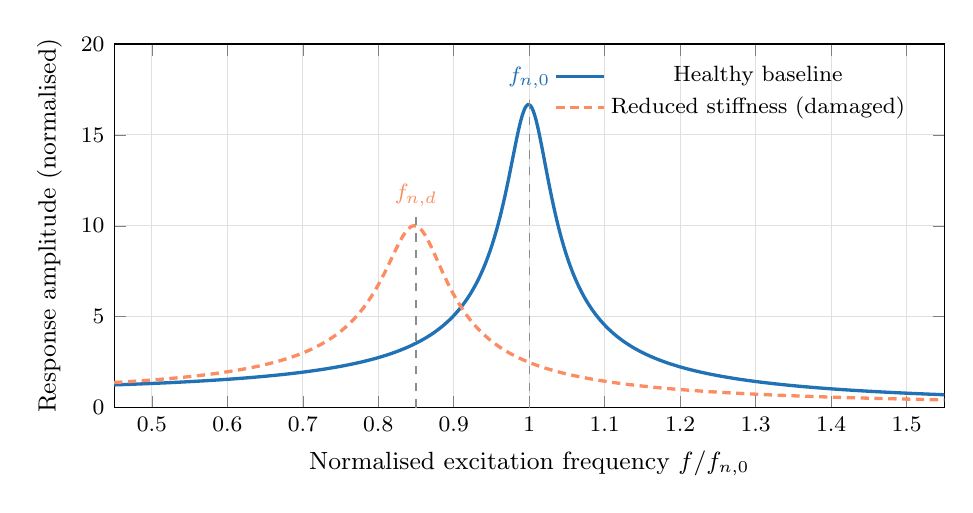
\begin{tikzpicture}
\begin{axis}[
  width=\linewidth, height=6.2cm,
  xlabel={Normalised excitation frequency $f/f_{n,0}$},
  ylabel={Response amplitude (normalised)},
  domain=0.45:1.55, samples=300,
  xmin=0.45, xmax=1.55, ymin=0, ymax=20,
  legend pos=north east, legend style={font=\footnotesize, draw=none, fill=none},
  tick label style={font=\footnotesize}, label style={font=\small},
  grid=major, grid style={black!12}
]
\addplot[elsB2, very thick, smooth] {1/sqrt((1-x^2)^2 + (2*0.03*x)^2)};
\addlegendentry{Healthy baseline}
\addplot[elsC2, very thick, densely dashed, smooth] {1/sqrt((1-(x/0.85)^2)^2 + (2*0.05*(x/0.85))^2)};
\addlegendentry{Reduced stiffness (damaged)}
\draw[black!45, dashed] (axis cs:1,0) -- (axis cs:1,17);
\draw[black!45, dashed] (axis cs:0.85,0) -- (axis cs:0.85,10.5);
\node[font=\footnotesize, elsB2, anchor=south] at (axis cs:1.0,17) {$f_{n,0}$};
\node[font=\footnotesize, elsC2, anchor=south] at (axis cs:0.85,10.5) {$f_{n,d}$};
\end{axis}
\end{tikzpicture}
\caption{Schematic frequency-response curve of a single vibration mode under harmonic (rotating-unbalance) excitation. A loss of stiffness lowers the natural frequency from $f_{n,0}$ to $f_{n,d}$ and, with the increased energy dissipation typical of damage, lowers and broadens the resonance peak. The curves are illustrative and do not represent measured data.}
\label{fig:frf}
\end{figure}

\begin{table}[htbp]
\centering
\footnotesize
\caption{Positioning of the proposed framework against representative digital-twin and machine-learning monitoring works. \checkmark{}~addressed; $\sim$~partial; --~not addressed. DT: physics-based (finite-element) digital twin; ML: machine learning for damage detection; AUT: embedded/autonomous interpretation; MAT: explicit L0--L5 self-awareness scale; GOV: governed healthy-baseline update; STL: steel-specific demonstrator or protocol.}
\label{tab:positioning}
\begin{tabularx}{\linewidth}{@{}X cccccc@{}}
\toprule
\textbf{Work} & \textbf{DT} & \textbf{ML} & \textbf{AUT} & \textbf{MAT} & \textbf{GOV} & \textbf{STL} \\
\midrule
Structural digital-twin framework \citep{chiachio2022structural}        & \checkmark & $\sim$     & $\sim$     & --         & --         & --         \\
Deep-learning and digital-twin SHM \citep{zou2026deep}                  & \checkmark & \checkmark & $\sim$     & --         & --         & --         \\
Edge--fog--cloud autonomous SHM \citep{li2025edge}                      & \checkmark & $\sim$     & \checkmark & --         & --         & --         \\
Digital-twin SHM with data governance \citep{mariniello2025enhancing}   & \checkmark & \checkmark & $\sim$     & --         & $\sim$     & --         \\
ML damage location on steel \citep{parisi2022steel}                     & --         & \checkmark & $\sim$     & --         & --         & \checkmark \\
Digital-twin-driven ML framework \citep{karyofyllas2025dtml}            & \checkmark & \checkmark & $\sim$     & --         & --         & $\sim$     \\
Physics-guided ML and FEM updating \citep{zhang2021physicsguided}       & $\sim$     & \checkmark & --         & --         & --         & $\sim$     \\
\textbf{This work (Self-Aware Steel Structure)}                         & \checkmark & \checkmark & \checkmark & \checkmark & \checkmark & \checkmark \\
\bottomrule
\end{tabularx}
\end{table}


\section{The Structural Cognition paradigm and Self-Aware Steel Structures}\label{sec:paradigm}

Conventional structural health monitoring (SHM) is defined as the process of implementing a damage detection strategy for engineering infrastructure: observing a structure over time through periodically spaced response measurements, extracting damage-sensitive features, and statistically analysing those features to determine the current state of system health \citep{farrar2013shm}. In its mature, deployed form this process is overwhelmingly \textit{extrospective}: instrumentation records strains, accelerations, temperatures and displacements, transmits them to a data acquisition system, and stores them for later interrogation by an engineer or an offline algorithm. The structure itself remains a passive load-resisting object, and the cognitive act of converting measurements into an assessment of integrity occurs elsewhere, asynchronously, and usually under human supervision. This is consistent with Axiom IVa of SHM, that sensors cannot measure damage, which establishes that feature extraction and statistical classification are always required to convert sensor data into damage information \citep{farrar2013shm,farrar2007introduction}. Conventional practice satisfies this axiom by delegating interpretation outside the structure; the paradigm proposed here satisfies it by embedding interpretation within the monitored system itself. Table~\ref{tab:conv-vs-aware} contrasts the two approaches across the dimensions that matter for autonomous assessment.

We define \textbf{Structural Cognition} as the capacity of an instrumented structure to perceive, process, interpret and report its own mechanical state through a permanent, bidirectional coupling between its physical instantiation and a continuously updated digital representation. A \textbf{Self-Aware Steel Structure} is the realisation of this capacity in a steel system: a structure that does not merely transmit raw data but maintains an internal, evolving model of what constitutes its own healthy behaviour, evaluates incoming responses against that model, recognises deviations attributable to stiffness change, connection loosening or progressive damage, and autonomously communicates the resulting assessment. Cognition here is operational rather than metaphorical: it denotes a closed loop in which the structure's measured dynamics are continuously confronted with model-based and data-based expectations, and the residual between expectation and observation is itself the carrier of self-knowledge. This framing is consistent with the data-and-model fusion view of the digital twin, in which predictions are a principled combination of physics models and streaming measurement data \citep{brunton2019data,chiachio2022structural}, and with the physical basis that natural frequencies, mode shapes and damping depend only on mass and stiffness \citep{chopra2017dynamics,cook2002fea}, so that a change in stiffness can produce detectable changes in modal parameters under adequate excitation, sensing and observability conditions.

\subsection{Levels of structural self-awareness}\label{subsec:levels}

To make the paradigm operational and measurable, we propose a six-level model of structural self-awareness, ordered by the depth of internal interpretation a structure performs on its own response. The levels are cumulative: each presupposes the capabilities of those below it. Fig.~\ref{fig:levels} depicts the progression from a passive member to an autonomous agent, and Table~\ref{tab:levels} gives the formal definition of each level together with its mapping onto the Rytter damage-identification hierarchy.

\begin{itemize}
\item \textbf{L0, Passive.} A purely load-resisting member with no instrumentation. Condition is established only by periodic human inspection; the two-state comparison on which damage assessment depends \citep{farrar2013shm} exists, if at all, in the inspector's judgement.
\item \textbf{L1, Sensing.} A distributed sensor network acquires and transmits raw signals (strain, acceleration, temperature, displacement, inclination). This is the level at which most deployed SHM systems terminate: data are stored and transmitted, but the structure performs no interpretation. It corresponds to \textit{data acquisition}, the second part of the statistical pattern recognition paradigm \citep{farrar2013shm}.
\item \textbf{L2, Perception (feature extraction).} The system reduces high-dimensional raw streams to low-dimensional, damage-sensitive features: natural frequencies, mode shapes, damping ratios, dominant modes obtained by SVD/POD, or autoencoder latent variables \citep{farrar2013shm,brunton2019data}. This satisfies Axiom IVa by performing the feature extraction that sensors alone cannot, and it embeds \textit{data normalisation} so that benign operational and environmental variability, notably temperature-induced stiffness change, is separated from response changes caused by damage \citep{farrar2013shm,figueiredo2010machine}.
\item \textbf{L3, Interpretation (diagnosis).} The structure decides whether its current behaviour is consistent with its healthy baseline, and, where it is not, localises and classifies the anomaly. Unsupervised novelty/outlier detection, trained on healthy data only, flags abnormal conditions; supervised classifiers (Random Forest, SVM, ANN) assign damage type and level \citep{farrar2013shm,naser2023ml,sohn2003statistical}. Diagnosis is the act of forming an internal verdict about state, minimising false-positive and false-negative indications \citep{farrar2013shm}.
\item \textbf{L4, Prognosis.} The structure estimates the implications of its diagnosed state for future performance and remaining useful life, fusing the diagnosed condition with model-based predictions of how the identified change propagates. This is \textit{damage prognosis} in the SHM sense \citep{farrar2013shm} and depends on a predictive digital twin able to extrapolate beyond the observed condition \citep{zou2026deep}.
\item \textbf{L5, Autonomous reporting and decision.} The structure communicates its self-assessment without prompting and, where authorised, triggers actions: alarms, maintenance requests, load restrictions, or re-calibration of its own baseline. This is the level at which the structure becomes an agent supporting condition-based and predictive maintenance \citep{farrar2013shm,naser2023ml}, closing the loop between physical event and digital decision.
\end{itemize}

\subsection{Mapping onto the Rytter damage-identification hierarchy}\label{subsec:rytter}

The self-awareness levels are deliberately aligned with the established Rytter hierarchy of damage identification, which orders the questions a diagnostic system can answer by increasing knowledge of the damage state: existence, location, type, severity (extent) and prognosis \citep{farrar2013shm}. \textbf{L2} establishes the feature basis on which any of these questions can be posed. \textbf{L3} answers \textit{existence} and \textit{location}, which Axiom III holds can be addressed in an unsupervised mode, and then advances to \textit{type} and \textit{severity}, which Axiom III holds generally require supervised learning \citep{farrar2013shm,wangcha2022unsupervised}. \textbf{L4} corresponds directly to \textit{prognosis}, the estimation of remaining safe or useful life. \textbf{L5} adds no new diagnostic question but operationalises the answers by communicating and acting upon them autonomously. The hierarchy therefore supplies the diagnostic semantics of structural cognition, while the levels supply its architectural and behavioural semantics: the first describes \textit{what} is known about the damage, the second \textit{how autonomously the structure itself comes to know and act upon it}.

\subsection{The perceive--process--interpret--report loop and the physical--digital link}\label{subsec:loop}

The transition from L1 to L5 is not a sequence of discrete products but a continuous loop executed in place. The \textbf{perceive} stage corresponds to L1 sensing across the heterogeneous, distributed network, with data fusion across same-type arrays (for example, strain gauges) and across heterogeneous channels (acceleration, temperature, inclination) to improve fidelity \citep{farrar2013shm}. The \textbf{process} stage (L2) compresses and normalises these streams into stable features. The \textbf{interpret} stage (L3 and L4) confronts the features with the structure's internal expectation of itself, a finite-element-derived modal and harmonic baseline \citep{chopra2017dynamics,cook2002fea} continuously corrected by data through the digital twin \citep{brunton2019data}, and converts residuals into diagnosis and prognosis. The \textbf{report} stage (L5) returns the verdict to operators and, where permitted, to the structure's own control of baselines and alarms.

What distinguishes this loop from conventional SHM is the permanence and bidirectionality of the physical--digital link. In conventional practice the link is intermittent and one-directional: data flow from structure to archive, and human interpretation flows back only at inspection intervals. In a Self-Aware Steel Structure the link is unbroken, since the digital twin is continuously fed by streaming data and continuously returns updated expectations and verdicts \citep{brunton2019data,li2025edge}, so that interpretation becomes a property the structure carries with it rather than a service performed upon it. The fundamental premise that damage requires a comparison between two system states \citep{farrar2013shm} is thereby internalised: the healthy baseline ceases to be an archived record and becomes a living, model-and-data representation against which the structure perpetually measures itself. This is an enrichment of SHM, not a replacement: every level rests on the statistical pattern recognition paradigm and the SHM axioms \citep{farrar2013shm}. Structural Cognition is the claim that these well-established processes, when embedded, closed and made autonomous, transform a passive member into a structure that understands, and reports, its own condition.

\begin{table}[htbp]
\centering
\caption{Conventional structural health monitoring compared with the proposed Self-Aware Steel Structure.}
\label{tab:conv-vs-aware}
\begin{tabularx}{\linewidth}{@{}l X X@{}}
\toprule
\textbf{Aspect} & \textbf{Conventional SHM} & \textbf{Self-Aware Steel Structure} \\
\midrule
Role of the structure   & Passive load-resisting member            & Cognitive, self-interpreting system \\
Locus of interpretation & Offline, performed by a human expert     & Embedded and autonomous \\
Healthy baseline        & Archived measurement records             & Living finite-element-and-data digital twin \\
Use of data             & Acquisition, storage and transmittal     & Perception, diagnosis and prognosis \\
Temporal coverage       & Periodic or event-triggered              & Continuous and real-time \\
Output                  & Raw data and inspection reports          & Autonomous integrity assessment \\
Maintenance paradigm    & Time-based inspection                    & Condition-based and predictive \\
\bottomrule
\end{tabularx}
\end{table}

\begin{figure}[htbp]
\centering
\resizebox{\linewidth}{!}{%
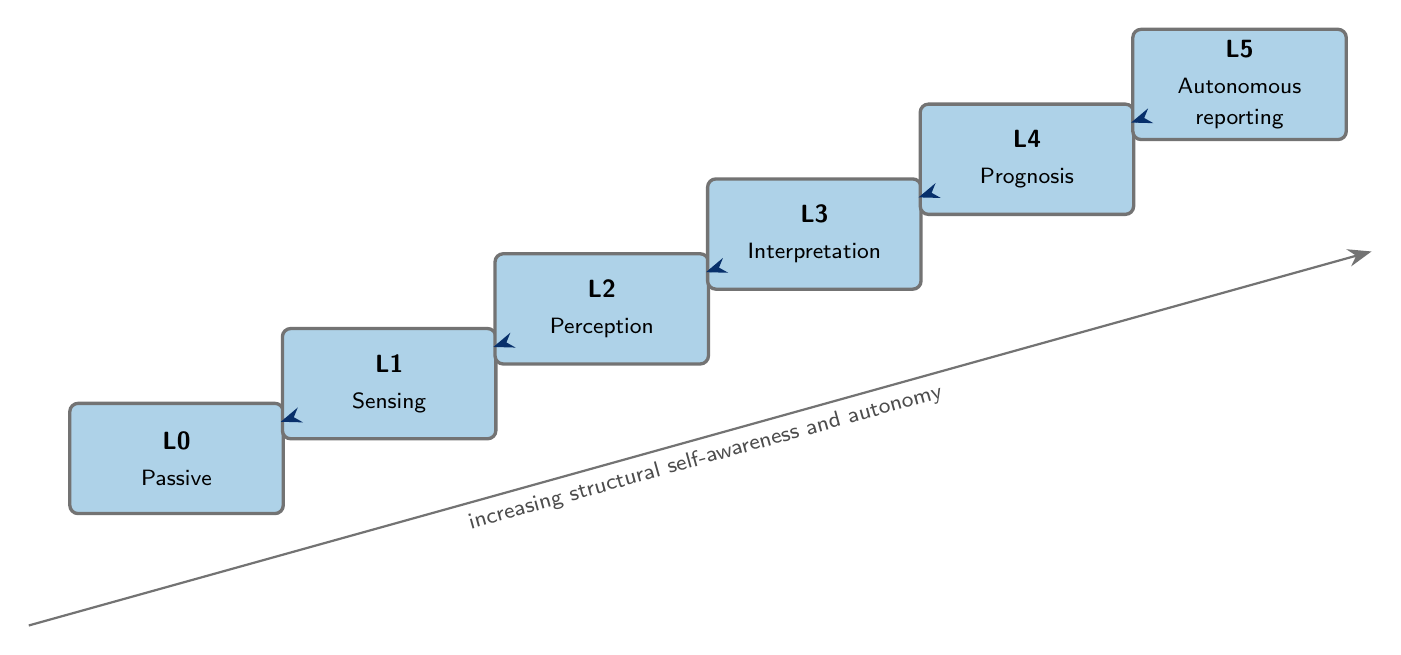
\begin{tikzpicture}[
  every node/.style={font=\small\sffamily},
  lvl/.style={rectangle, rounded corners=3pt, draw=black!55, very thick,
               fill=elsB3!55, text width=2.5cm, minimum height=1.4cm, align=center, inner sep=3pt},
  up/.style={-{Stealth[length=2.6mm]}, very thick, elsB1}
]
  \foreach \i/\lab/\cap in {0/L0/Passive, 1/L1/Sensing, 2/L2/Perception,
                            3/L3/Interpretation, 4/L4/Prognosis, 5/L5/{Autonomous reporting}} {
     \node[lvl] (n\i) at (\i*2.7, \i*0.95) {\textbf{\lab}\\[2pt]\footnotesize \cap};
  }
  \foreach \i [evaluate=\i as \j using int(\i+1)] in {0,1,2,3,4} {
     \draw[up] (n\i) -- (n\j);
  }
  \draw[-{Stealth[length=3mm]}, thick, black!55]
       ($(n0.south west)+(-0.5,-1.4)$) -- ($(n5.south east)+(0.3,-1.4)$)
       node[midway, below, sloped, font=\footnotesize\sffamily, black!70]
       {increasing structural self-awareness and autonomy};
\end{tikzpicture}}
\caption{The six levels of structural self-awareness, from a passive member (L0) to a structure that autonomously reports and acts upon its own state (L5). Each level presupposes the capabilities of those below it. The mapping to learning techniques and to the Rytter hierarchy is detailed in Table~\ref{tab:levels}.}
\label{fig:levels}
\end{figure}

\begin{table}[htbp]
\centering
\caption{Levels of structural self-awareness and their mapping to the Rytter damage-identification hierarchy.}
\label{tab:levels}
\begin{tabularx}{\linewidth}{@{}c X p{2.5cm} X@{}}
\toprule
\textbf{Level} & \textbf{Capability} & \textbf{Rytter stage} & \textbf{Enabling technique} \\
\midrule
L0 & Passive member; condition established by inspection & --             & Visual inspection \\
L1 & Acquires and transmits raw signals                 & --             & Distributed sensor network \\
L2 & Extracts damage-sensitive features                 & (precondition) & SVD/PCA, modal identification, autoencoder latents \\
L3 & Detects, locates and classifies anomalies          & Existence, location, type, severity & Novelty detection; Random Forest, SVM, ANN \\
L4 & Estimates remaining useful life                    & Prognosis & Predictive digital twin; LSTM networks \\
L5 & Communicates and acts on its self-assessment       & --             & Decision logic; condition-based maintenance \\
\bottomrule
\end{tabularx}
\end{table}


\section{Reference architecture of a self-aware steel structure}\label{sec:architecture}

The transition from a passively monitored steel frame to a self-aware structure requires more than additional sensors; it requires an organizing architecture in which raw physical measurements are progressively transformed into interpretable knowledge about the structural state. We propose a five-layer reference architecture (sensing, data acquisition and signal conditioning, physics-based digital twin, cognition, and decision and reporting), summarized in Fig.~\ref{fig:arch}, that maps directly onto the statistical pattern recognition (SPR) paradigm for SHM \citep{farrar2013shm} while extending it with a continuously updated digital twin and an embedded cognition layer. Each layer consumes the output of the one below it and returns feedback to the layers beneath, so that the architecture operates as a closed perceive--process--interpret--report loop rather than a one-way data pipeline. The physics-based and data-driven components are not alternatives but co-operating elements of a hybrid, physics-informed system \citep{brunton2019data}, in which law-based models supply features and constraints to the machine-learning layer, and the machine-learning layer in turn supplies updated parameters and residuals back to the physics model \citep{chiachio2022structural,zou2026deep}.

\subsection{Sensing layer}\label{subsec:sensing}

The sensing layer realizes the data-acquisition concerns of the SPR paradigm: selection of sensor types, number and locations \citep{farrar2013shm}. For the planned SHS braced-frame testbed, a heterogeneous, spatially distributed sensor network is foreseen, comprising electrical strain gauges (local strain and, through the constitutive law, stress), triaxial accelerometers (dynamic response for modal identification), temperature sensors (for thermal compensation and data normalisation), displacement sensors (global deflections), and inclinometers (global stability and rigid-body rotation). The planned channels and their monitoring roles are listed in Table~\ref{tab:sensors}. This heterogeneity is deliberate: data fusion across both homogeneous arrays (for example, a distributed strain-gauge array) and complementary modalities (acceleration combined with temperature and operational parameters) improves damage-detection fidelity and supports separation of benign variability from genuine damage \citep{farrar2013shm}. The number and placement of sensors are not chosen ad hoc but determined by preliminary numerical analysis of the finite-element baseline, which identifies the degrees of freedom most informative about the target modes and the most likely damage scenarios. This is consistent with sparse and optimal sensor-placement strategies (for example, QR- and DEIM-based selection and gappy POD) that allow reconstruction of the full response field from a limited number of measurements \citep{brunton2019data,tan2020sensorplacement,hassani2023sensorplacement}, and it respects the axiomatic principle that the length and time scales of the damage of interest dictate the required sensing-system properties \citep{farrar2013shm}. A fundamental constraint inherited at this layer is that sensors cannot measure damage directly; they measure response quantities from which damage information must subsequently be extracted \citep{farrar2013shm}.

\subsection{Data acquisition and signal-conditioning layer}\label{subsec:acquisition}

The acquisition layer converts the analog physical quantities sensed above into clean, synchronized and meaningful digital streams. A central DAQ system continuously samples the strain, acceleration, temperature, displacement and inclination channels at rates sufficient to resolve the highest natural frequencies of interest, in keeping with the snapshot-pair sampling requirements of data-driven modal methods \citep{brunton2019data}. Signal conditioning includes amplification, anti-alias filtering, bridge completion and excitation for the strain gauges, and time synchronization across channels so that mode shapes can be reconstructed from phase-consistent measurements. This layer also performs the data normalisation, cleansing, compression and fusion processes that are inherent to steps two through four of the SPR paradigm \citep{farrar2013shm}. Temperature channels are used here for thermal compensation, so that response changes caused by environmental variation, the canonical example being temperature-induced stiffness change, are not later misinterpreted as damage and reported as false positives \citep{farrar2013shm,figueiredo2010machine}. Temperature is the variability source this layer measures and removes directly; humidity, wind and randomly varying operational loads perturb the response as well, and because the testbed does not instrument them, they are left to the statistical normalization performed downstream in the cognition layer. Dimensionality reduction begins at this stage: the singular value decomposition and principal component analysis provide a numerically stable, data-driven means of compressing high-dimensional strain and acceleration streams into a few dominant coherent structures that define a low-dimensional baseline of healthy behavior \citep{brunton2019data}.

\subsection{Physics-based digital-twin layer}\label{subsec:digitaltwin}

At the core of the architecture is a finite-element model (FEM) that serves as the structure's physical baseline. The FEM idealizes the braced frame using bar and beam/frame elements appropriate to skeletal steel structures, with element stiffness matrices assembled into the global stiffness matrix and with explicit modeling decisions, notably the representation of bolted beam-column connections as semi-rigid rotational springs whose stiffness is an updatable parameter bounded by the pinned and rigid idealizations, treated as part of the mathematical model that the analysis actually solves \citep{cook2002fea}. The model supports the full suite of analyses required to establish baseline behavior: static analysis $[\mathbf{K}]\{\mathbf{D}\}=\{\mathbf{R}\}$, modal analysis via the undamped eigenproblem $([\mathbf{K}]-\omega^2[\mathbf{M}])\{\mathbf{D}\}=\{\mathbf{0}\}$ yielding natural frequencies and mode shapes, harmonic (frequency-response) analysis for the planned rotating-unbalance excitation, which the FE literature explicitly recognizes as a harmonic source applied by rotating machinery \citep{cook2002fea}, and transient response history. Mass is represented through consistent or lumped mass matrices and energy dissipation through Rayleigh proportional damping, $[\mathbf{C}]=a[\mathbf{M}]+b[\mathbf{K}]$ \citep{cook2002fea,chopra2017dynamics}. This model becomes a digital twin once it is continuously fed by sensor data and its predictions are compared in real time against measured responses \citep{chiachio2022structural,zou2026deep}. Because natural frequencies and mode shapes depend only on mass and stiffness \citep{chopra2017dynamics}, any stiffness loss, from progressive damage or bolted-connection loosening, manifests as a measurable shift in modal parameters and as a growing deviation between predicted and observed response. Model updating closes the gap: experimentally identified parameters are fed back to recalibrate the FEM, embodying the principle that finite-element analysis is simulation rather than reality and must be correlated with experiment \citep{cook2002fea}. Reduced-order representations, obtained through static condensation and substructuring \citep{cook2002fea} or POD-Galerkin projection \citep{brunton2019data}, make this comparison fast enough for real-time, streaming operation \citep{li2025edge}.

\subsection{Cognition layer}\label{subsec:cognition}

The cognition layer is where the structure interprets, rather than merely records, its own state, and it is organized along the Rytter damage-state hierarchy of existence, location, type, severity and prognosis \citep{farrar2013shm}. Perception is achieved through single-class models trained only on healthy data: autoencoders learn an unsupervised latent representation of normal behavior and flag abnormal conditions through growing reconstruction error \citep{brunton2019data}, while LSTM recurrent networks, used in a self-supervised forecasting mode, learn the healthy temporal evolution of the vibration and strain streams and flag deviations in sequential response \citep{brunton2019data,naser2023ml}. These novelty- and outlier-detection approaches answer the existence (and often location) questions in an unsupervised mode, consistent with the SHM axiom that existence and location can be found without labels whereas type and severity generally require supervision \citep{farrar2013shm,sohn2003statistical,wangcha2022unsupervised}. Diagnosis and damage-level classification are then handled by supervised learners, Random Forest, Support Vector Machines and Artificial Neural Networks, trained on labeled scenarios such as minor/major/collapse-style categories \citep{naser2023ml,parisi2022steel}. Because labeled damaged-state data are scarce when intentionally damaging a high-value structure is impractical \citep{farrar2013shm}, the validated FEM doubles as a data source: parametric simulation generates augmented, hybrid (real-plus-simulated) training sets \citep{naser2023ml}. The features consumed here are explicitly physics-derived: natural frequencies, mode shapes, damping ratios (estimable by half-power bandwidth, \citealp{chopra2017dynamics}), residuals between FEM prediction and measurement, and SVD/DMD modal descriptors \citep{brunton2019data}, so that physics and machine learning co-operate rather than compete \citep{avci2021review}.

\subsection{Decision and reporting layer}\label{subsec:decision}

The uppermost layer converts the cognition layer's quantified damage state into autonomous, actionable communication, realizing the operational-evaluation purpose of the SPR paradigm of life-safety and economic justification \citep{farrar2013shm}. Diagnostic and prognostic outputs are framed to minimize false-positive and false-negative diagnoses, whose costs may be weighted asymmetrically \citep{farrar2013shm}, and are made interpretable and auditable through explainable-ML techniques such as permutation feature importance, SHAP and partial-dependence plots that trace each alarm back to physically checkable indicators \citep{naser2023ml}. The structure thereby reports its own integrity, supporting the shift from time-based to condition-based and predictive maintenance \citep{farrar2013shm,mariniello2025enhancing}. Feedback flows downward, but under explicit governance, so that slow degradation is not silently absorbed into the notion of health. The reference healthy baseline is immutable and versioned; any adaptation of the working baseline, the FEM or the cognition models is conditioned on independent confirmation, monitored for concept drift, gated by human approval for safety-critical changes, and reversible through a rollback mechanism. Only validated, non-damaging changes, such as recalibration for a new operational or environmental regime, are propagated. This governed feedback closes the perceive--process--interpret--report loop that distinguishes a self-aware steel structure from conventional data-collecting SHM.

\begin{table}[htbp]
\centering
\caption{Planned distributed sensor network for the demonstrator testbed.}
\label{tab:sensors}
\begin{tabularx}{\linewidth}{@{}l l X@{}}
\toprule
\textbf{Sensor} & \textbf{Measured quantity} & \textbf{Monitoring purpose} \\
\midrule
Electrical strain gauges  & Strains (and stresses)   & Local force paths and quasi-static load effects; strain-based features \\
Triaxial accelerometers   & Accelerations            & Natural frequencies, mode shapes and damping (modal identification) \\
Temperature sensors       & Temperature              & Thermal compensation and environmental normalisation of signals \\
Displacement transducers  & Displacements            & Global and local deflections \\
Inclinometers             & Rotations and tilt       & Global stability and rigid-body drift \\
\bottomrule
\end{tabularx}
\end{table}


\section{Experimental methodology and demonstrator testbed}\label{sec:methodology}

This section describes the planned demonstrator and the integrated experimental and numerical methodology through which the Self-Aware Steel Structure concept will be instantiated and assessed. No experiments have yet been performed; what follows is the proposed protocol. The strategy deliberately couples a physical testbed, a continuously updated finite-element representation and the machine-learning layer described in the preceding sections, so that the structure is not merely instrumented but is enabled to interpret and report its own mechanical state.

\subsection{Physical demonstrator}\label{subsec:demonstrator}

The demonstrator will be a three-dimensional braced frame fabricated from square hollow structural steel sections (SHS). This configuration is chosen because it is representative of skeletal steel systems widely used in industrial buildings, warehouses, elevated platforms and modular construction, where bar- and beam-type idealizations are appropriate \citep{cook2002fea}. Beam-to-column connections will be bolted and idealized as pinned, while global lateral stability will be provided exclusively by diagonal bracing. The arrangement isolates two well-defined and physically meaningful damage scenarios, loss of bracing axial stiffness and loosening of bolted connections, both of which manifest as changes in material or geometric properties, boundary conditions or system connectivity, and therefore satisfy the formal definition of damage as a change of state adversely affecting performance \citep{farrar2013shm}. A loosened bolted connection, in particular, alters connectivity and typically increases energy dissipation, producing a measurable rise in vibrational damping that the monitoring system is designed to capture. The complete instrumented demonstrator and its coupling to the digital-twin loop are shown in Fig.~\ref{fig:testbed}.

\subsection{Instrumentation and sensor-placement strategy}\label{subsec:instrumentation}

A distributed, heterogeneous sensor network will be deployed. The planned channels comprise electrical resistance strain gauges (local strains and, via the constitutive relation, stresses); triaxial accelerometers (dynamic response for modal identification); temperature sensors (thermal compensation and operational or environmental normalization); displacement transducers (static and quasi-static deflections); and inclinometers (global stability and drift). Sensor positions will not be chosen ad hoc but will be selected from a preliminary numerical analysis of the FEM. Candidate locations will be ranked by their sensitivity to the targeted modal quantities and damage scenarios, so that accelerometers are placed where the lower mode shapes exhibit large modal amplitude and strain gauges where the damage-sensitive members carry significant force. This model-informed placement reflects the principle that sensing-system requirements are dictated by the length and time scales of the damage of interest, and that distributed arrays plus heterogeneous data fusion improve detection fidelity \citep{farrar2013shm}. It is also consistent with established computational sensor-placement strategies and optimization algorithms developed for SHM \citep{tan2020sensorplacement,hassani2023sensorplacement}. The full channel list, the measured quantity and the placement rationale for each sensor type are summarized in Table~\ref{tab:sensors}. All signals will be continuously acquired, synchronized and time-stamped by a central data-acquisition (DAQ) system, supplying the streams of strain, acceleration, displacement, temperature and inclination from which the higher-level features, natural frequencies, mode shapes, damping ratios and stiffness indicators, will be derived.

\subsection{Excitation system and frequency sweeps}\label{subsec:excitation}

Controlled dynamic loading will be applied by a rotating-unbalance excitation system: a variable-speed electric motor driving an eccentric mass rigidly attached to the frame. This is the textbook mechanism for applying harmonic excitation to full-scale structures via rotating machinery \citep{cook2002fea}, with a force amplitude proportional to the square of the excitation frequency, $p(t)=m_e\,e\,\omega^2\sin\omega t$ \citep{chopra2017dynamics}. Because the force scales with $\omega^2$, the device is well suited to dynamic rather than static testing. The motor speed will be swept across a range that brackets the lower natural frequencies of the frame, allowing the steady-state frequency-response curve to be traced; its peaks locate the resonant frequencies and their sharpness encodes damping through the half-power bandwidth \citep{chopra2017dynamics}. By exciting at and near resonance, the test campaign will deliberately amplify the response in order to reveal modal shifts, resonance migration and changes in resonant amplitude induced by introduced stiffness changes or damage. The physical basis is the direct coupling $\omega_n=\sqrt{k/m}$, whereby any stiffness loss is observable as a downward shift in natural frequency and an increase in measured damping \citep{chopra2017dynamics}.

\subsection{Finite-element model and parameter identification}\label{subsec:femodel}

A finite-element model will reproduce the static and dynamic behavior of the demonstrator. SHS members will be discretized with beam/frame elements assembled into the global stiffness matrix $[\mathbf{K}]$; mass will be represented by a consistent (or, where appropriate, lumped) mass matrix $[\mathbf{M}]$, and energy dissipation by Rayleigh proportional damping $[\mathbf{C}]=a[\mathbf{M}]+b[\mathbf{K}]$ \citep{cook2002fea}. The model will incorporate section geometry, measured material properties, idealized boundary conditions and connection flexibility, with the pinned or rigid idealization of bolted joints treated explicitly as a modeling decision to be reconciled with measurement. Four analysis types will establish the baseline: static analysis $[\mathbf{K}]\{\mathbf{D}\}=\{\mathbf{R}\}$; modal analysis via the undamped eigenproblem $([\mathbf{K}]-\omega_n^2[\mathbf{M}])\{\boldsymbol{\phi}\}=\{\mathbf{0}\}$, yielding the baseline natural frequencies and mode shapes; harmonic (frequency-response) analysis to predict steady-state amplitude versus excitation frequency under the rotating-unbalance load; and transient analysis for non-stationary events \citep{cook2002fea,chopra2017dynamics}. Recognizing that finite-element analysis is simulation, not reality \citep{cook2002fea}, the model will be calibrated against the undamaged structure: experimentally identified modal parameters will be used to update stiffness, connection-flexibility and damping parameters so that the numerical baseline faithfully represents the as-built healthy state. Comparable modal identification and system-identification campaigns on full-scale steel members support the feasibility of this calibration step \citep{yu2024steelbridge}.

\subsection{Digital-twin integration and deviation indicators}\label{subsec:dtintegration}

The validated FEM will serve as the kernel of a digital twin continuously fed by the live sensor streams \citep{chiachio2022structural}. At each monitoring step, measured responses (strains, frequencies, mode shapes, damping, displacements) will be compared in real time against the twin's predictions for the current operating and environmental condition, with temperature channels used to normalize benign variability so that environmental effects are not mistaken for damage \citep{farrar2013shm}. Deviations will be quantified through statistical indicators and performance parameters: residuals between measured and predicted features, control-chart-style thresholds, and distance metrics on the modal and feature space, providing the quantitative bridge between physical state and digital representation \citep{sohn2003statistical}. Persistent, statistically significant deviations from the healthy baseline will then be passed to the machine-learning layer for novelty detection, classification and severity assessment, closing the perceive--process--interpret--report loop that defines Structural Cognition \citep{zou2026deep}.

\subsection{Six-step methodology}\label{subsec:sixstep}

The study will proceed through the following sequential and partly iterative steps:

\begin{enumerate}
    \item \textbf{Develop the finite-element model} of the SHS braced frame, including geometry, materials, connection flexibility and boundary conditions, and run static, modal, harmonic and transient analyses to establish baseline behavior.
    \item \textbf{Build the instrumented physical structure}, fabricating and erecting the bolted, braced 3D frame as the experimental demonstrator.
    \item \textbf{Install and calibrate the distributed sensor network} (strain gauges, accelerometers, temperature sensors, displacement transducers, inclinometers) at the numerically selected positions, and integrate the central DAQ.
    \item \textbf{Run static and dynamic tests}, including rotating-unbalance frequency sweeps near the natural frequencies, on the healthy structure and under controlled, reversible damage scenarios (bracing stiffness reduction, bolted-connection loosening).
    \item \textbf{Implement the digital twin and integrate real-time data}, performing continuous FEM-versus-measurement comparison with statistical deviation indicators and environmental normalization.
    \item \textbf{Train, validate and apply the AI layer} (supervised and unsupervised models) for autonomous structural-integrity assessment, mapping deviations to the existence, location, type and severity of damage.
\end{enumerate}

To make this plan auditable rather than merely descriptive, Table~\ref{tab:params} consolidates the parameters that fully define the campaign: geometry, material, connections, sensor count and placement, sampling and filtering, excitation, quantified damage levels, the model-updating procedure, the alarm thresholds, and the train/validation/test partition. These values are deliberately presented as a specification to be finalised with the as-built structure; the present paper fixes the protocol and the quantities to be reported, not measured results.

\begin{figure}[htbp]
\centering
\resizebox{\linewidth}{!}{%
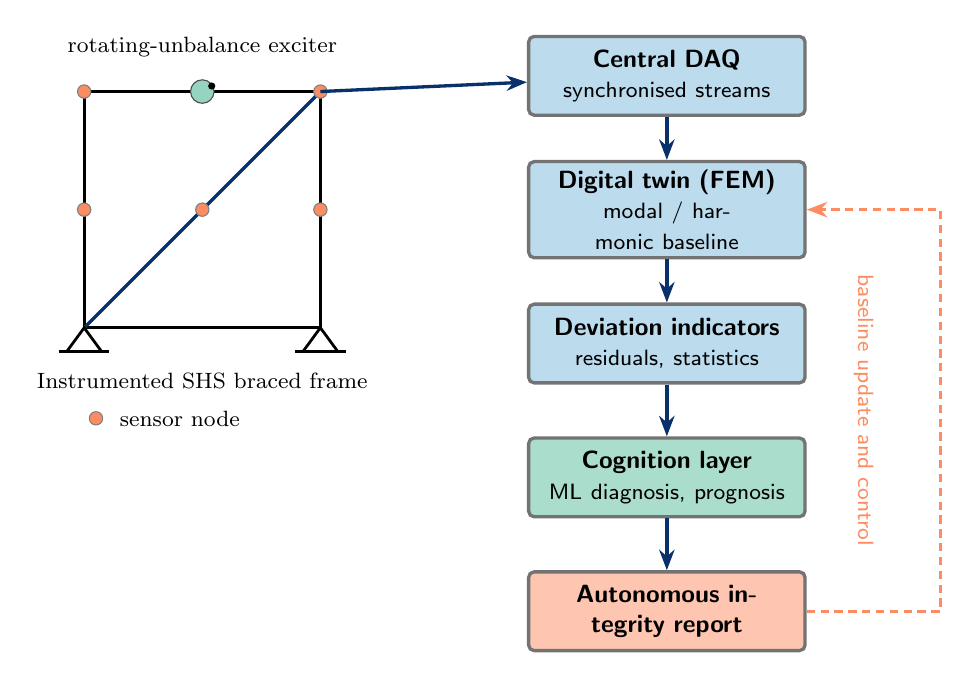
\begin{tikzpicture}[
  every node/.style={font=\small\sffamily},
  box/.style={rectangle, rounded corners=2pt, draw=black!55, very thick, fill=elsB3!45,
              text width=3.3cm, minimum height=1.0cm, align=center, inner sep=3pt},
  cogb/.style={rectangle, rounded corners=2pt, draw=black!55, very thick, fill=elsC1!55,
              text width=3.3cm, minimum height=1.0cm, align=center, inner sep=3pt},
  repb/.style={rectangle, rounded corners=2pt, draw=black!55, very thick, fill=elsC2!50,
              text width=3.3cm, minimum height=1.0cm, align=center, inner sep=3pt},
  sensor/.style={circle, fill=elsC2, draw=black!50, inner sep=1.7pt},
  arr/.style={-{Stealth[length=2.6mm]}, very thick, elsB1},
  fb/.style={-{Stealth[length=2.6mm]}, very thick, densely dashed, elsC2}
]
  % ---- physical frame (left) ----
  \coordinate (bl) at (0,0.4);   \coordinate (br) at (3,0.4);
  \coordinate (tl) at (0,3.4);   \coordinate (tr) at (3,3.4);
  \draw[line width=1.2pt] (bl) -- (tl) -- (tr) -- (br);
  \draw[line width=1.2pt] (bl) -- (br);
  \draw[line width=1.2pt, elsB1] (bl) -- (tr);
  \foreach \p in {bl,br} {
     \draw[line width=1pt] ($(\p)+(-0.22,-0.3)$) -- (\p) -- ($(\p)+(0.22,-0.3)$);
     \draw[line width=1pt] ($(\p)+(-0.32,-0.3)$) -- ($(\p)+(0.32,-0.3)$);
  }
  \node[circle, draw=black!70, fill=elsC1!70, inner sep=3pt] (mot) at (1.5,3.4) {};
  \fill[black] ($(mot)+(0.12,0.07)$) circle (1.3pt);
  \node[font=\footnotesize, anchor=south] at (1.5,3.72) {rotating-unbalance exciter};
  \node[sensor] at (0,1.9){};  \node[sensor] at (3,1.9){};  \node[sensor] at (1.5,1.9){};
  \node[sensor] at (0,3.4){};  \node[sensor] at (3,3.4){};
  \node[font=\footnotesize, anchor=north] at (1.5,-0.05) {Instrumented SHS braced frame};
  \node[sensor] (leg) at (0.15,-0.75){};
  \node[font=\footnotesize, anchor=west] at (0.33,-0.75) {sensor node};
  % ---- vertical digital pipeline (right) ----
  \node[box]  (daq)  at (7.4, 3.6) {\textbf{Central DAQ}\\ \footnotesize synchronised streams};
  \node[box]  (twin) at (7.4, 1.9) {\textbf{Digital twin (FEM)}\\ \footnotesize modal / harmonic baseline};
  \node[box]  (dev)  at (7.4, 0.2) {\textbf{Deviation indicators}\\ \footnotesize residuals, statistics};
  \node[cogb] (cog)  at (7.4,-1.5) {\textbf{Cognition layer}\\ \footnotesize ML diagnosis, prognosis};
  \node[repb] (rep)  at (7.4,-3.2) {\textbf{Autonomous integrity report}};
  \draw[arr] (tr) -- (daq);
  \draw[arr] (daq) -- (twin);
  \draw[arr] (twin) -- (dev);
  \draw[arr] (dev) -- (cog);
  \draw[arr] (cog) -- (rep);
  \draw[fb] (rep.east) -- ++(1.7,0) |- (twin.east);
  \node[rotate=-90, anchor=south, font=\footnotesize\sffamily, elsC2] at (9.65,-0.65)
        {baseline update and control};
\end{tikzpicture}}
\caption{Schematic of the planned demonstrator and its digital counterpart. The instrumented square-hollow-section (SHS) braced frame is excited by a variable-speed rotating-unbalance device; synchronised sensor streams feed a central data-acquisition system and the finite-element-based digital twin, whose predictions are compared with measurement to produce deviation indicators. The cognition layer converts these into an autonomous integrity report, which in turn updates the healthy baseline, closing the perceive--process--interpret--report loop.}
\label{fig:testbed}
\end{figure}

\begin{table}[htbp]
\centering
\caption{Experimental specification of the demonstrator. The quantities below define an auditable protocol; symbolic values are to be finalised with the as-built structure, and no value is measured yet.}
\label{tab:params}
\begin{tabularx}{\linewidth}{@{}l X l@{}}
\toprule
\textbf{Group} & \textbf{Parameter} & \textbf{Specification} \\
\midrule
Geometry        & SHS section $b\times t$; bay length; total height                                   & to be finalised \\
Material         & Steel grade; Young's modulus $E$; density $\rho$                                    & to be finalised \\
Connections      & Bolt grade and preload; semi-rigid joint rotational stiffness (bounded by pinned and rigid) & to be finalised \\
Sensors          & Number and position of strain, acceleration, temperature, displacement, inclination & FE sensitivity analysis \\
Acquisition      & Sampling rate $f_s$; anti-alias cut-off; window length                              & to be finalised \\
Excitation       & Eccentric mass $m_e$; eccentricity $e$; rotation range $\Omega$                     & to be finalised \\
Damage scenarios & Bracing stiffness-reduction levels; bolt-loosening torque levels                    & quantified \\
FEM updating     & Updated parameters; objective function; algorithm                                   & to be finalised \\
Alarm logic      & Deviation indicator; threshold; control-chart limits                                & to be finalised \\
Data partition   & Grouping unit; external test set                                                    & by test/scenario/condition \\
\bottomrule
\end{tabularx}
\end{table}


\section{Machine-learning strategy for autonomous damage detection}\label{sec:ml}

The machine-learning (ML) layer is the component that raises the proposed system from conventional Structural Health Monitoring (SHM), which typically terminates at data acquisition and storage, to genuine Structural Cognition, in which the structure interprets its own responses. This layer is organized as a statistical pattern-recognition pipeline whose four canonical procedures are operational evaluation, data acquisition, feature extraction, and statistical modelling for feature discrimination \citep{farrar2013shm,farrar2007introduction}. Fig.~\ref{fig:mlpipeline} shows how this pipeline maps onto the Rytter damage stages, from existence through prognosis. Within that pipeline, the central methodological commitment of the present framework is that ML does not operate on raw signals alone but on damage-sensitive features and on residuals computed against the calibrated digital twin, so that physics and data are fused rather than opposed \citep{brunton2019data}. The strategy is deliberately tiered, because the single most important constraint in any field SHM deployment is data scarcity: damaged-state data from a high-value structure are rarely available, so the architecture must function in a predominantly data-poor regime while remaining able to exploit labelled scenarios when they exist \citep{farrar2013shm,naser2023ml,avci2021review}.

\subsection{Damage-sensitive feature extraction}\label{subsec:features}

Feature extraction converts sensor data into low-dimensional quantities that are highly sensitive to structural condition and, ideally, insensitive to benign variability. Two complementary feature families are extracted. The first is a set of physics-based modal features: natural frequencies, mode shapes, and modal damping ratios, identified from the triaxial-accelerometer network under the rotating-unbalance excitation. These are physically interpretable because, for the idealized braced frame, the natural frequencies and modes depend only on the mass and stiffness distribution, so any stiffness loss, bracing degradation, or bolted-connection loosening manifests as a measurable downward shift in frequency, a distortion of the mode shape, and, where energy dissipation increases, a rise in measured damping \citep{chopra2017dynamics,farrar2013shm}. The second family is data-driven features obtained by compressing the distributed strain and acceleration streams: the singular value decomposition / principal component analysis yields the dominant spatial modes of healthy operation, and dynamic mode decomposition extracts spatio-temporal coherent structures, each with an associated oscillation frequency and growth/decay rate, directly from experimental snapshots without requiring the governing equations \citep{brunton2019data}. A third, and arguably the most discriminative, feature is the residual between the measured response and the digital-twin prediction. Because the finite-element-based twin produces baseline modal parameters and time histories, prediction errors and statistical indicators on these residuals act as features whose growth flags a divergence between the physical structure and its validated model \citep{brunton2019data,farrar2013shm}.

\subsection{Environmental and operational normalization}\label{subsec:normalization}

A feature is useful for damage detection only after benign operational and environmental variability has been separated from genuine condition change; otherwise temperature-driven stiffness variation or changes in excitation amplitude are mistaken for damage, producing false-positive alarms \citep{farrar2013shm,figueiredo2010machine}. The planned temperature sensors provide the auxiliary measurements needed for this normalization, supplying thermal compensation of the strain channels and allowing modal features to be conditioned on temperature. Temperature is the confounder most directly measured and compensated, but it is not the only one. Humidity, wind buffeting and randomly varying operational loads also shift natural frequencies and damping; because the testbed instruments temperature rather than these quantities, their effect is handled statistically, by comparing features at similar points of the operational cycle and conditioning the healthy model on the inferred operational and environmental state \citep{figueiredo2010machine}. Normalization is treated as both a physical correction (thermal compensation of raw signals) and a statistical one (comparing features measured at similar points of the operational cycle, and conditioning the healthy model on the measured environmental state). Channel-specific care is required during fusion: tree ensembles are largely insensitive to scaling, whereas distance- and gradient-based learners (SVM, neural networks, PCA-derived features) are sensitive and require consistent normalization across the heterogeneous strain, acceleration, temperature, and displacement channels \citep{naser2023ml}.

\subsection{Unsupervised novelty detection (the data-poor default)}\label{subsec:unsupervised}

Because only healthy-state data are generally available, the default operating mode is unsupervised novelty/outlier detection: a model of the single healthy class is constructed, and incoming data are tested for consistency with that class \citep{farrar2013shm,wangcha2022unsupervised}. The primary tool is an autoencoder trained exclusively on healthy multi-sensor data; it learns a compact latent representation of normal behaviour, and its reconstruction error provides a natural, continuously evaluated anomaly indicator that rises when the structure departs from the learned baseline \citep{brunton2019data}. A linear autoencoder reduces to the SVD/PCA subspace, which makes the method interpretable and links the deep and classical formulations \citep{brunton2019data}. Complementary classical detectors provide low-parameter alternatives suited to streaming deployment: sequential probability ratio tests accumulate evidence across successive samples before declaring a change \citep{sohn2003statistical}, while outlier analysis based on Mahalanobis distance and density- or isolation-based methods offers distribution- and density-driven alternatives \citep{naser2023ml}. This route answers Rytter stage~1 (existence) and, when the spatially distributed sensor array localizes the anomalous response, contributes to stage~2 (location); it is subject to the axiomatic trade-off between damage sensitivity and noise-rejection capability, which governs threshold selection \citep{farrar2013shm}.

\subsection{Supervised classification (when labelled or simulated-damage data exist)}\label{subsec:supervised}

When damage classes can be labelled, most realistically from simulated-damage scenarios rather than from physical destruction of the testbed, supervised classifiers add localization and severity estimation. Random Forest, an ensemble of decision trees aggregated by majority voting, is non-parametric, insensitive to feature scaling, and pairs naturally with feature-importance analysis; Support Vector Machines separate damage classes by margin-maximizing hyperplanes with linear or radial-basis kernels; and Artificial Neural Networks, trained by back-propagation, capture more complex nonlinear mappings between features and damage state \citep{naser2023ml}. These supervised methods address Rytter stages~3 and~4 (type and severity), classifying conditions along an ordinal scale such as healthy / minor / major damage, consistent with the SHM axiom that existence and location are reachable unsupervised but type and severity generally require supervised learning \citep{farrar2013shm,naser2023ml,parisi2022steel}. Deployed studies confirm the maturity of this route for steel and infrastructure assets: supervised deep networks have classified the condition of bridge steel bearings \citep{wangsu2023steelbearing} and have detected and categorised damage across large, heterogeneous field datasets \citep{arya2021roaddamage}, illustrating the scale at which the supervised branch can operate once labelled data are available.

\subsection{Temporal modelling for progressive damage and bolt-loosening}\label{subsec:temporal}

Bolted-connection loosening and progressive stiffness loss are inherently time-evolving, and they are the damage mechanisms most directly relevant to the bolted SHS braced frame; loosening alters connectivity and adds energy dissipation, observable as drift in frequency and damping over time \citep{farrar2013shm}. Long Short-Term Memory (LSTM) recurrent networks are therefore used to model the temporal structure of the continuously acquired strain and vibration series, learning the healthy temporal evolution and forecasting expected response so that slow deviations, rather than single-sample outliers, are detected and trended \citep{brunton2019data,naser2023ml}. This supports incipient-fault detection and feeds the prognosis-oriented Rytter stage~5.

\subsection{Training, validation, evaluation, and explainability}\label{subsec:training}

Data scarcity is addressed by exploiting the validated finite-element model as a controlled data generator: parametric simulation of damage scenarios (localized stiffness reductions, bracing degradation, connection-flexibility changes) produces labelled cases that are compiled into a hybrid real-plus-simulated dataset for supervised training, with the explicit caveat that experimental data remain preferred and synthetic data require validation \citep{naser2023ml,cook2002fea}. Accordingly, any preliminary results obtained on this finite-element-generated, self-labelled set are reported as a specification of the validation protocol and its target metrics rather than as evidence of field performance, which only physically induced damage can establish. To avoid leakage between temporally adjacent windows of the same test, validation uses grouped (blocked) partitioning, in which all windows from a given test, damage scenario and operating or environmental condition are kept together in a single fold; generalisation is then assessed on an external test set of unseen scenarios and conditions rather than on randomly shuffled samples, and overfitting or underfitting is monitored across these grouped folds \citep{naser2023ml}. Performance is reported with several independent indicators rather than a single score, including the confusion matrix, ROC, precision, recall, F1, and balanced accuracy for classification, together with error and residual metrics for regression, while statistical models are explicitly tuned to balance false-positive and false-negative diagnoses according to their differing safety and economic costs \citep{farrar2013shm,naser2023ml}. To make autonomous integrity assessment trustworthy, decisions are accompanied by explainability, using permutation feature importance and SHAP, so that the features driving a damage indication can be checked for physical plausibility against the modal and residual quantities defined above \citep{naser2023ml}. The complete technique-to-stage mapping, summarized in Table~\ref{tab:mlmethods}, runs as follows: SVD/PCA, DMD, and twin-residual features supply the cognitive substrate; autoencoder and outlier analysis realize unsupervised perception (existence and location); Random Forest, SVM, and ANN realize supervised interpretation (type and severity); and LSTM realizes temporal reasoning toward prognosis. Together these methods advance the structure through successive Structural-Cognition levels rather than leaving it at passive data acquisition \citep{farrar2013shm,brunton2019data,naser2023ml}.

\begin{figure}[htbp]
\centering
\resizebox{\linewidth}{!}{%
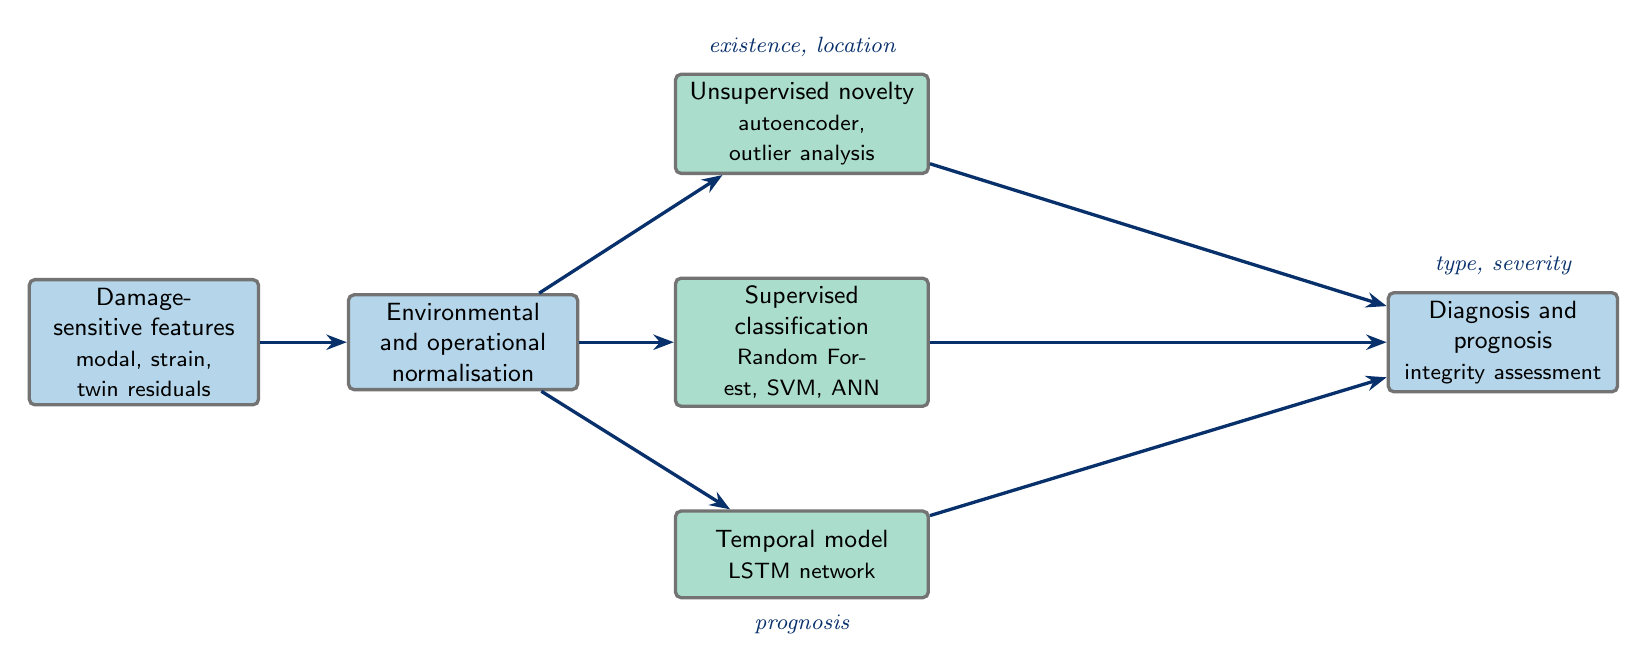
\begin{tikzpicture}[
  every node/.style={font=\small\sffamily},
  io/.style={rectangle, rounded corners=2pt, draw=black!55, very thick, fill=elsB3!50,
             text width=2.7cm, minimum height=1.1cm, align=center, inner sep=3pt},
  br/.style={rectangle, rounded corners=2pt, draw=black!55, very thick, fill=elsC1!55,
             text width=3.0cm, minimum height=1.1cm, align=center, inner sep=3pt},
  arr/.style={-{Stealth[length=2.6mm]}, very thick, elsB1}
]
  \node[io] (feat) {Damage-sensitive features\\ \footnotesize modal, strain, twin residuals};
  \node[io, right=1.1cm of feat] (norm) {Environmental and operational normalisation};
  \node[br, above right=1.5cm and 1.2cm of norm] (uns) {Unsupervised novelty\\ \footnotesize autoencoder, outlier analysis};
  \node[br, right=1.2cm of norm] (sup) {Supervised classification\\ \footnotesize Random Forest, SVM, ANN};
  \node[br, below right=1.5cm and 1.2cm of norm] (tmp) {Temporal model\\ \footnotesize LSTM network};
  \node[io, right=5.8cm of sup] (out) {Diagnosis and prognosis\\ \footnotesize integrity assessment};
  \draw[arr] (feat) -- (norm);
  \draw[arr] (norm) -- (uns);
  \draw[arr] (norm) -- (sup);
  \draw[arr] (norm) -- (tmp);
  \draw[arr] (uns) -- (out);
  \draw[arr] (sup) -- (out);
  \draw[arr] (tmp) -- (out);
  \node[font=\footnotesize\itshape, elsB1, anchor=south] at ($(uns.north)+(0,0.08)$) {existence, location};
  \node[font=\footnotesize\itshape, elsB1, anchor=north] at ($(tmp.south)+(0,-0.08)$) {prognosis};
  \node[font=\footnotesize\itshape, elsB1, anchor=south] at ($(out.north)+(0,0.08)$) {type, severity};
\end{tikzpicture}}
\caption{Machine-learning pipeline of the cognition layer. Damage-sensitive features are normalised against operational and environmental variability, then routed to an unsupervised branch (novelty detection), a supervised branch (damage classification) and a temporal branch (progressive-damage tracking). Each branch is annotated with the Rytter stages it addresses; the technique-to-stage mapping is summarised in Table~\ref{tab:mlmethods}.}
\label{fig:mlpipeline}
\end{figure}

\begin{table}[htbp]
\centering
\caption{Machine-learning methods mapped to the damage-identification task and the Structural Cognition levels.}
\label{tab:mlmethods}
\begin{tabularx}{\linewidth}{@{}X l l c@{}}
\toprule
\textbf{Method} & \textbf{Learning mode} & \textbf{Damage task (Rytter)} & \textbf{Level} \\
\midrule
SVD/PCA and DMD              & Feature extraction          & Substrate            & L2 \\
Autoencoder                  & Unsupervised                & Existence, location  & L2--L3 \\
Outlier analysis / SPRT      & Unsupervised                & Existence            & L3 \\
Random Forest                & Supervised                  & Type, severity       & L3 \\
Support Vector Machine       & Supervised                  & Type, severity       & L3 \\
Artificial Neural Network    & Supervised                  & Type, severity       & L3 \\
LSTM network                 & Sequential / self-supervised & Prognosis           & L4 \\
\bottomrule
\end{tabularx}
\end{table}


\section{Discussion: challenges, validation and outlook}\label{sec:discussion}

The Self-Aware Steel Structure framework proposed in this work is conceptually coherent and grounded in mature theory, yet its transition from paradigm to deployable practice raises a set of interdependent challenges that must be addressed candidly. The most fundamental caveat is that the framework is, at present, a proposal: the testbed, sensing network, digital twin and AI layer described above have not yet been built or experimentally validated. The arguments below should therefore be read as a critical roadmap rather than as evidence of demonstrated capability.

\textbf{Validation strategy.} A credible validation must proceed in stages and must distinguish between simulated and physically induced damage. The FEM provides a controllable environment in which stiffness reductions, connection releases and mass changes can be parametrically introduced to generate a hybrid dataset of healthy and damaged responses for initial AI training, a practice with clear precedent in using a validated finite element model as a data source \citep{naser2023ml}. FEM-simulated damage inherits the limitation that ``FEA is simulation, not reality'' \citep{cook2002fea}: even an accurate analysis of an inadequate mathematical model can disagree with the physical structure. Models trained predominantly on synthetic cases may therefore learn artefacts of the idealization, such as the particular connection-stiffness model adopted, rather than true structural physics, and real or experimental data are generally to be favored over purely synthetic data \citep{naser2023ml}. A classifier assessed only on cases that the finite-element model itself generated and labelled demonstrates class separability under the model's own assumptions, not performance on the physical structure; any preliminary numerical study is therefore reported as a specification of the validation protocol and the target metrics it will use, rather than as evidence of field capability. Physically induced damage, through controlled bolt loosening, added masses, or member removal in the bracing, is indispensable for closing this reality gap. Bolted-connection loosening is a particularly appropriate target because it alters system connectivity and adds energy dissipation, which typically manifests as a measurable increase in damping \citep{farrar2013shm,razi2013bolted,chelimilla2023looseness}, consistent with the documented precedent in which period lengthening accompanied stiffness reduction and increased damping at damaging amplitudes \citep{chopra2017dynamics}. The contrast between this self-interpreting workflow and conventional data-collecting monitoring is summarized in Table~\ref{tab:conv-vs-aware}. Validation must be grouped rather than randomly shuffled: folds must hold out whole \textit{tests}, damage \textit{scenarios} and \textit{operating conditions} together, rather than individual and possibly adjacent windows, while the class imbalance between abundant healthy and scarce damaged data is handled explicitly, to guard against the optimistic bias and overfitting that arise when training performance far exceeds testing performance \citep{naser2023ml,figueiredo2010machine}.

\textbf{Generalization across structures.} A model trained on one SHS braced frame encodes that structure's specific mass, stiffness and modal signature. Because natural frequencies and mode shapes depend only on mass and stiffness \citep{chopra2017dynamics}, they are intrinsically structure-specific, and a damage classifier learned on the testbed will not transfer directly to a differently configured frame. Generalization will likely require physics-informed features, such as modal parameters and prediction residuals against the structure's own digital twin, rather than raw signals, together with transfer-learning strategies \citep{naser2023ml,karaaslan2021attention} that adapt a pretrained model to a new structure using limited local data.

\textbf{Sensor reliability, cost and computation.} The distributed network of strain gauges, accelerometers, temperature, displacement and inclination sensors introduces an inherent cost-versus-fidelity trade-off in deployment \citep{farrar2013shm}. Sensors degrade, drift and fail, and ``sensors cannot measure damage'' directly: feature extraction and statistical classification are always required \citep{farrar2013shm}. Numerically driven sensor placement, supported by reduced-order modeling and sparse or optimal placement techniques \citep{brunton2019data,tan2020sensorplacement,hassani2023sensorplacement}, can reduce channel count while preserving observability, but introduces its own approximation. Real-time operation is constrained by the cost of repeatedly solving the eigenproblem and the harmonic and transient analyses, which is far greater than the static solution \citep{cook2002fea}; reduced-order models and data-driven modal decomposition (DMD) \citep{brunton2019data} are the natural mitigations, at the price of fidelity in higher modes.

\textbf{Uncertainty, interpretability and trust.} A self-aware structure that \textit{reports} its state must also report its confidence. Without data normalization separating benign operational and environmental variability from genuine damage, the system will produce false-positive indications \citep{farrar2013shm,figueiredo2010machine}. Temperature-induced stiffness change is the canonical confounder, and the thermal-compensation channel addresses it directly. It is not the only one, however: varying operational loads, wind and humidity also perturb the modal parameters, and since the testbed does not instrument these quantities, they have to be separated statistically rather than measured away. Conditioning the healthy model on the inferred operational state, instead of assuming that temperature exhausts the benign variability, is what keeps such effects from being read as damage. The axiomatic trade-off between damage sensitivity and noise rejection \citep{farrar2013shm} bounds what any algorithm can achieve. Engineer trust further demands interpretability: black-box classifiers should be accompanied by explainability tools such as permutation feature importance, SHAP and partial dependence plots, so that flagged anomalies map to physically checkable indicators \citep{naser2023ml}. Deep models also face generalizability and interpretability limits together with large-data requirements \citep{brunton2019data}.

\textbf{Standardization, integration and scalability.} For the paradigm to reach asset-management practice it must integrate with BIM and digital-asset workflows and adopt standardized data and damage-state semantics, for example the Rytter hierarchy of existence, location, type, severity and prognosis \citep{farrar2013shm}, so that autonomous outputs are interpretable across stakeholders \citep{chiachio2022structural,mariniello2025enhancing}. Scaling from a laboratory frame to in-service warehouses, platforms and modular structures multiplies environmental variability, connection count and uncontrolled excitation, where the rotating-unbalance source is replaced by ambient and operational loads \citep{he2022integrated}.

\textbf{Multimodal perception.} The framework developed here is deliberately vibration-based: perception, the digital twin and the cognition layer all operate on the dynamic response of the SHS frame, and the testbed carries no optical instrumentation. The five-layer architecture is nonetheless open at its sensing and cognition layers to complementary perception modalities. Vision-based deep learning is the most immediate of these: on infrastructure imagery, convolutional networks already detect and classify surface damage such as corrosion and cracking \citep{karaaslan2021attention,arya2021roaddamage}, and segmentation variants can localize such damage at the pixel level. A visual channel of this kind would observe surface and geometric damage that modal features reach only indirectly, and fusing a learned visual damage index with the modal and twin-residual features could corroborate an event across independent modalities. Bolted-connection loosening, for instance, would register as both an increase in damping and a localized change in the image of the joint. This multimodal route is left to future work: it requires its own camera network, annotated image datasets and trained models, none of which belongs to the present vibration-based specification.

\textbf{Limitations.} Beyond the absence of experimental validation, the framework relies on a single excitation mechanism and on modally observable damage types; and although the bolted connections are now represented as semi-rigid rotational springs rather than ideal pins, their stiffness still has to be identified experimentally before the numerical model can serve as a trusted baseline. The detectable damage size is inversely proportional to the excitation frequency range \citep{farrar2013shm}, which limits sensitivity to small or local flaws. These constraints define the agenda for the experimental program rather than negating the concept.


\section{Conclusions and future work}\label{sec:conclusions}

This paper introduced \textbf{Structural Cognition} as a new paradigm for steel structures and articulated its concrete embodiment, the \textbf{Self-Aware Steel Structure}: a structure able to perceive, process, interpret and continuously report its own mechanical state. The central argument is that conventional structural health monitoring, even when it delivers real-time measurement, largely stops at data acquisition and storage, leaving interpretation to periodic human analysis. Grounded in the statistical pattern recognition paradigm and the fundamental axioms of SHM \citep{farrar2013shm}, the proposed framework reframes the structure itself as the locus of interpretation. Rather than merely collecting strain, acceleration and temperature streams, a Self-Aware Steel Structure recognizes healthy behavior, identifies anomalies, detects stiffness loss and bolted-connection loosening, classifies damage severity, and autonomously communicates its condition along the Rytter hierarchy of existence, location, type, extent and prognosis.

The contribution is threefold. The \textbf{conceptual paradigm} distinguishes data-collecting SHM from a structure that interprets its own responses and maintains a permanent, bidirectional link to its digital representation. The \textbf{reference architecture} then layers a distributed multi-sensor network (strain gauges, triaxial accelerometers, temperature, displacement and inclinometer channels), a finite element baseline of static, modal, harmonic and transient behavior, a continuously updated digital twin, a machine-learning cognition layer, and a governed decision-and-reporting layer that issues autonomous assessments under explicit governance. This architecture is theoretically coherent: modal parameters depend only on mass and stiffness, so that damage can produce detectable shifts in natural frequencies, mode shapes and damping when excitation and observability are adequate \citep{chopra2017dynamics,cook2002fea}; data-driven dimensionality reduction and model discovery compress distributed signals into low-dimensional damage-sensitive features and a healthy baseline \citep{brunton2019data}; and supervised classifiers (Random Forest, SVM, ANN), unsupervised novelty detectors (autoencoders) and self-supervised temporal models (LSTM) map onto the SHM division between detecting damage and characterizing its type, severity and evolution \citep{farrar2013shm,naser2023ml,wangcha2022unsupervised}. Finally, the \textbf{six-step methodology} sequences FEM development, physical construction, sensor installation and calibration, static and dynamic testing, digital-twin integration, and AI training, validation and deployment into a structured, auditable engineering protocol.

The expected impact spans the lifecycle of steel infrastructure. By converting passive load-resisting members into self-interpreting systems, the framework promises improved \textbf{safety} through continuous, near-real-time condition screening; reduced \textbf{inspection cost} by shifting from time-based to condition-based and predictive maintenance; and increased \textbf{reliability} through traceable, physics-consistent damage indicators. Together these elements point toward \textbf{cognitive digital twins} and autonomous predictive-maintenance systems for the next generation of intelligent structures \citep{chiachio2022structural,zou2026deep}.

We emphasize that the methodology, testbed and AI layer described here are \textbf{planned}; no experiments have yet been performed, and the framework is offered as a conceptual and architectural proposal rather than a validated result. The concrete next steps are the following:

\begin{enumerate}
    \item \textbf{Build the three-dimensional braced SHS frame demonstrator} with bolted, semi-rigid connections, and instrument it at sensor positions selected by preliminary numerical analysis.
    \item \textbf{Develop and calibrate the finite element model}, establishing baseline modal and harmonic behavior and verifying it against independent solutions and experiment \citep{cook2002fea}.
    \item \textbf{Run the planned static and dynamic tests} using the variable-speed rotating-unbalance excitation to traverse natural frequencies and induce controlled, reversible stiffness changes.
    \item \textbf{Integrate the digital twin} with live sensor feeds and quantify deviations via statistical indicators.
    \item \textbf{Train, validate and deploy the AI cognition layer}, using rigorous metrics and cross-validation, addressing scarce damaged-state data through FE-augmented datasets, and incorporating explainability so that autonomous integrity assessments remain physically interpretable and trustworthy \citep{naser2023ml}.
\end{enumerate}

Demonstrating closed-loop structural cognition on this testbed is the immediate objective of future work.


%% ===================== Declarations =====================
\section*{CRediT authorship contribution statement}
\textbf{[First Author]:} Conceptualization, Methodology, Writing -- original draft.
\textbf{[Second Author]:} Conceptualization, Supervision, Writing -- review \& editing.

\section*{Declaration of competing interest}
The authors declare that they have no known competing financial interests or
personal relationships that could have appeared to influence the work reported in
this paper.

%% ===================== Bibliography =====================
\bibliographystyle{elsarticle-num}
\bibliography{references}

\end{document}
